%=========================================================
\section{Modelo de la interacción}	
\label{cap:modInteraccion}

En esta sección se describe el mapa de navegación y se presentan las pantallas del sistema. Estos mapas organizan y representan la estructura de interacción entre las diferentes pantallas y secciones disponibles para cada usuario. 
De igual manera, estos mapas de navegación ilustran las rutas de acceso para cada usuario según sus roles y permisos. Se detallan las páginas de inicio, y las conexiones entre módulos o funcionalidades principales que se pueden realizar dentro del sistema.

\subsection{Modelo de navegación}

La navegación entre pantallas para los 3 usuarios (alumno, docente y personal de seguridad) se detalla en los mapas presentados a continuación. Cada mapa describe las pantallas accesibles para cada tipo de usuario, así como las transiciones posibles entre ellas. Estas representaciones permiten visualizar de manera clara el flujo de interacción y las funcionalidades disponibles para cada perfil.

\begin{figure}[htbp]
	\begin{center}
			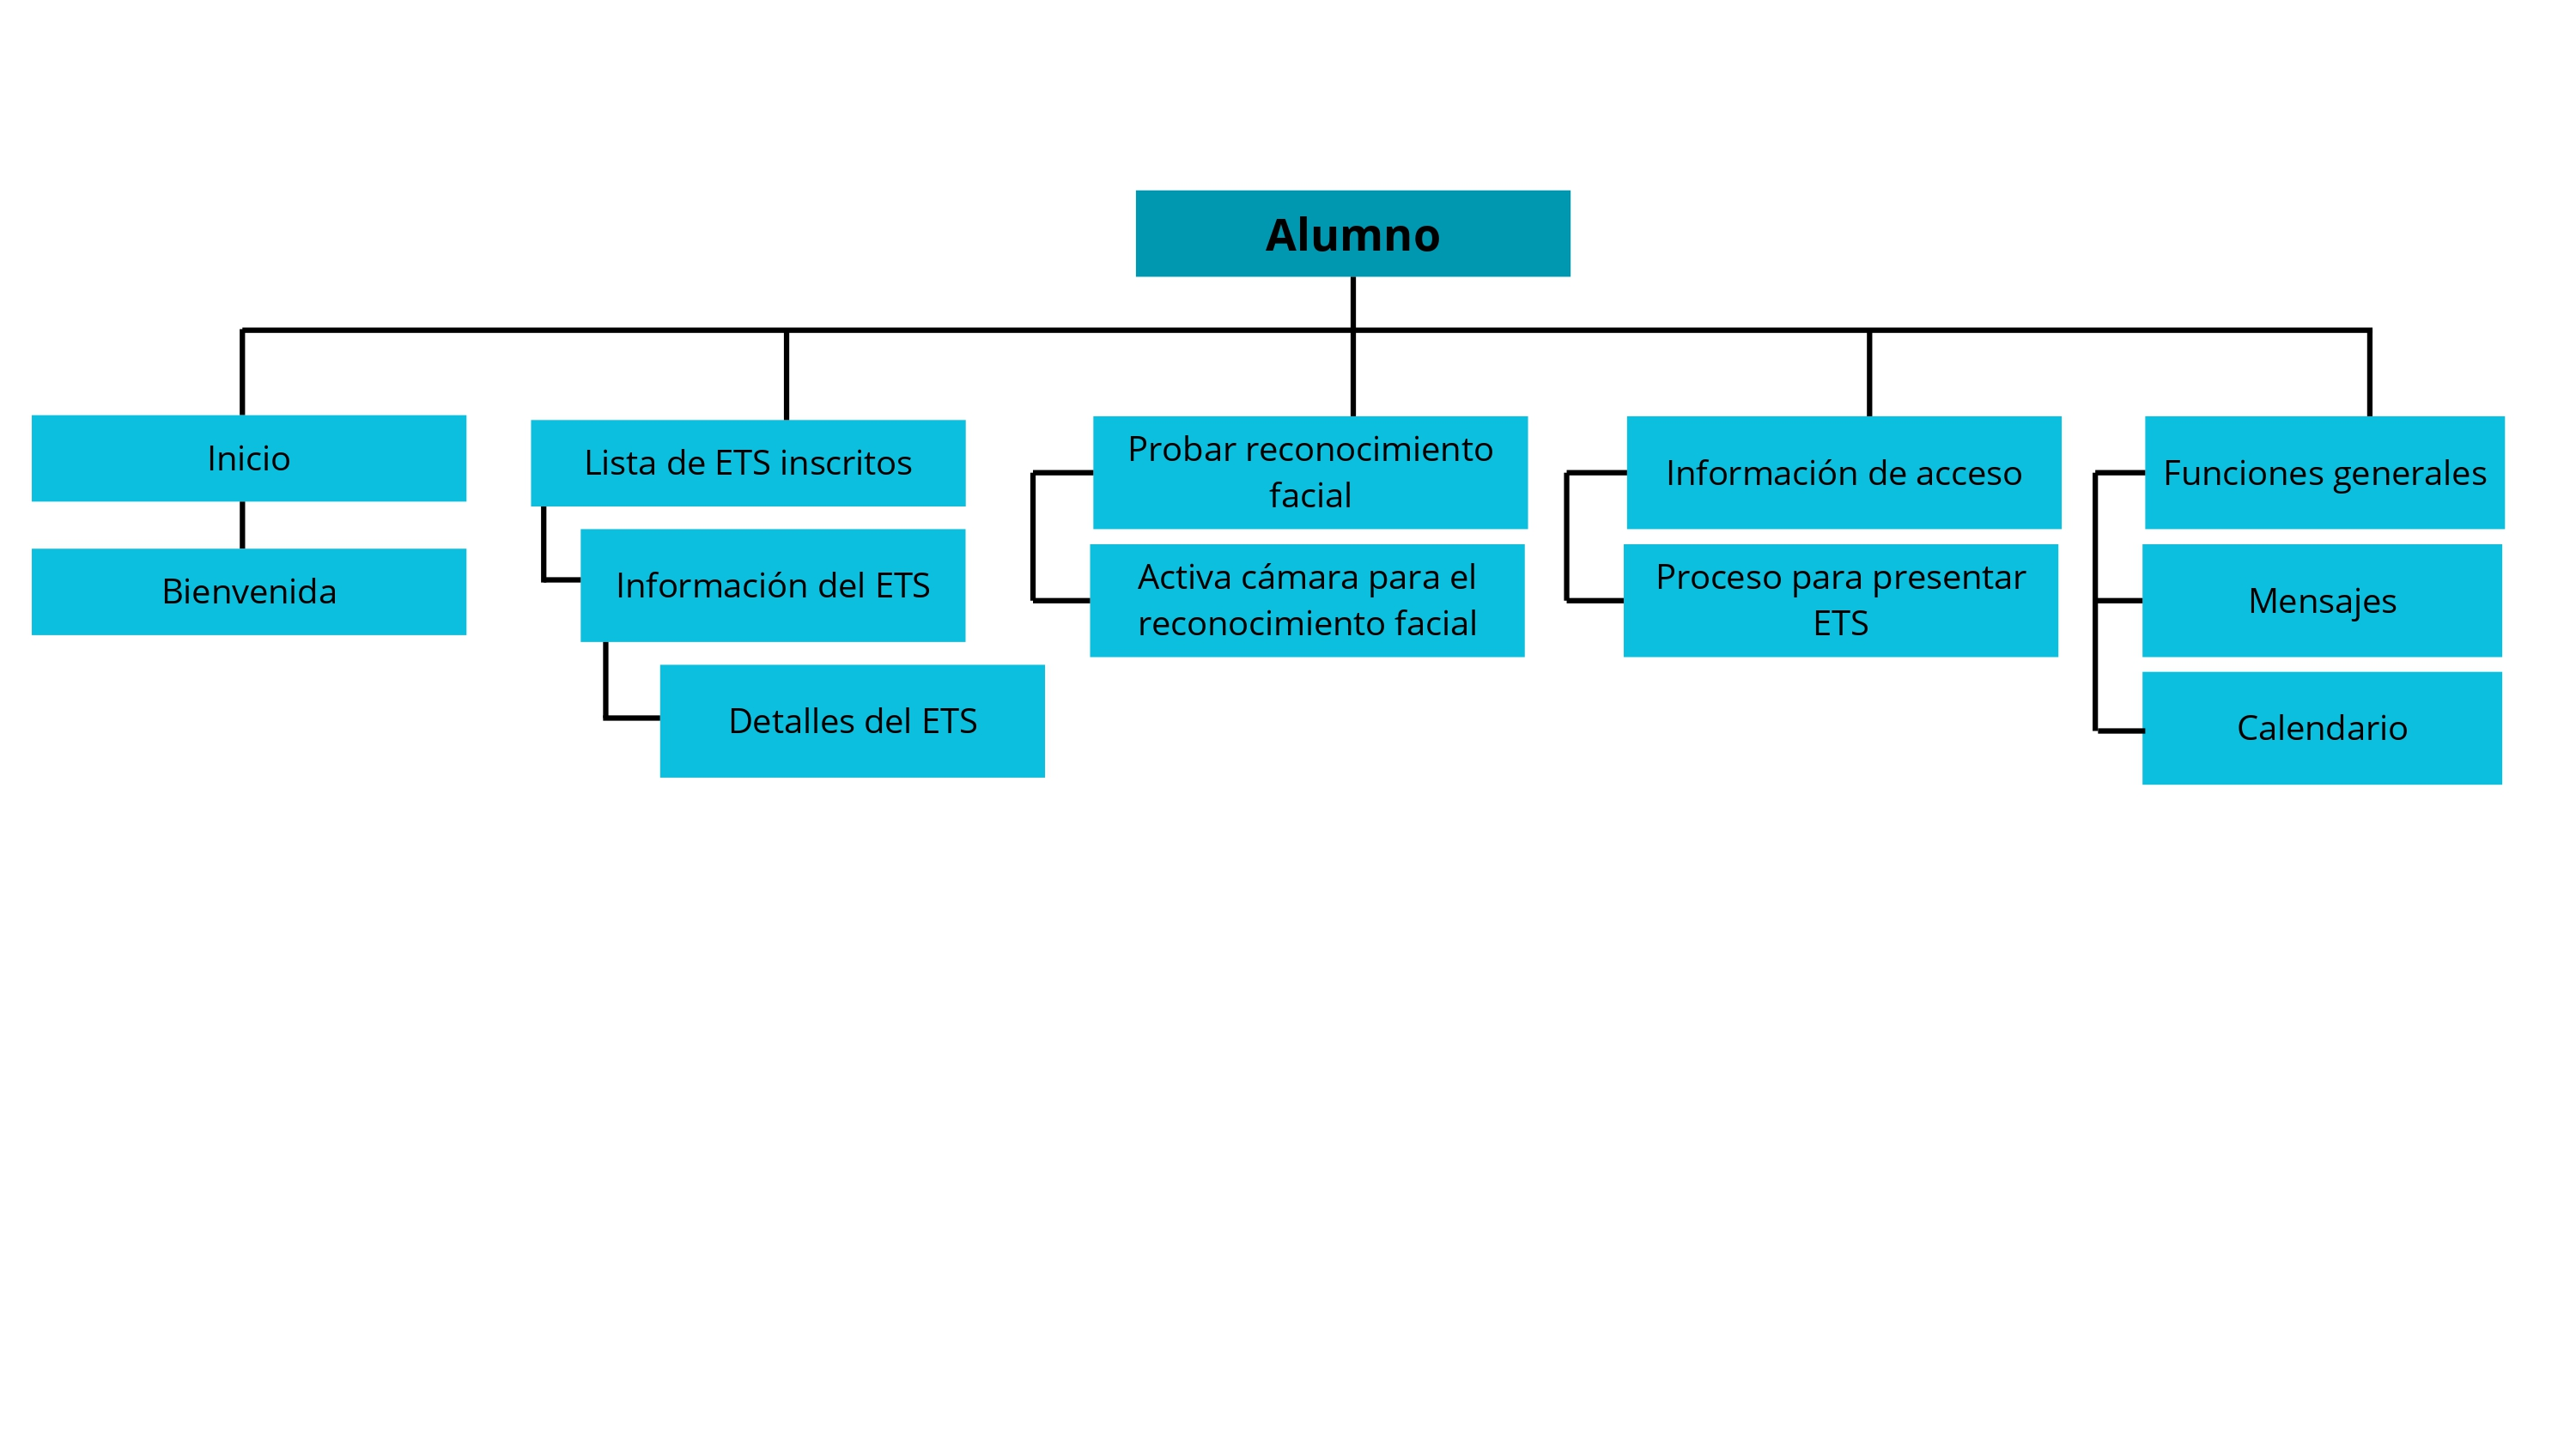
\includegraphics[width=1.0\textwidth]{images/alumno}
			\caption{Mapa de navegación del alumno}
			\label{fig:Mapa de navegación del alumno}
		\end{center}
\end{figure}

\clearpage

\begin{figure}[htbp]
	\begin{center}
		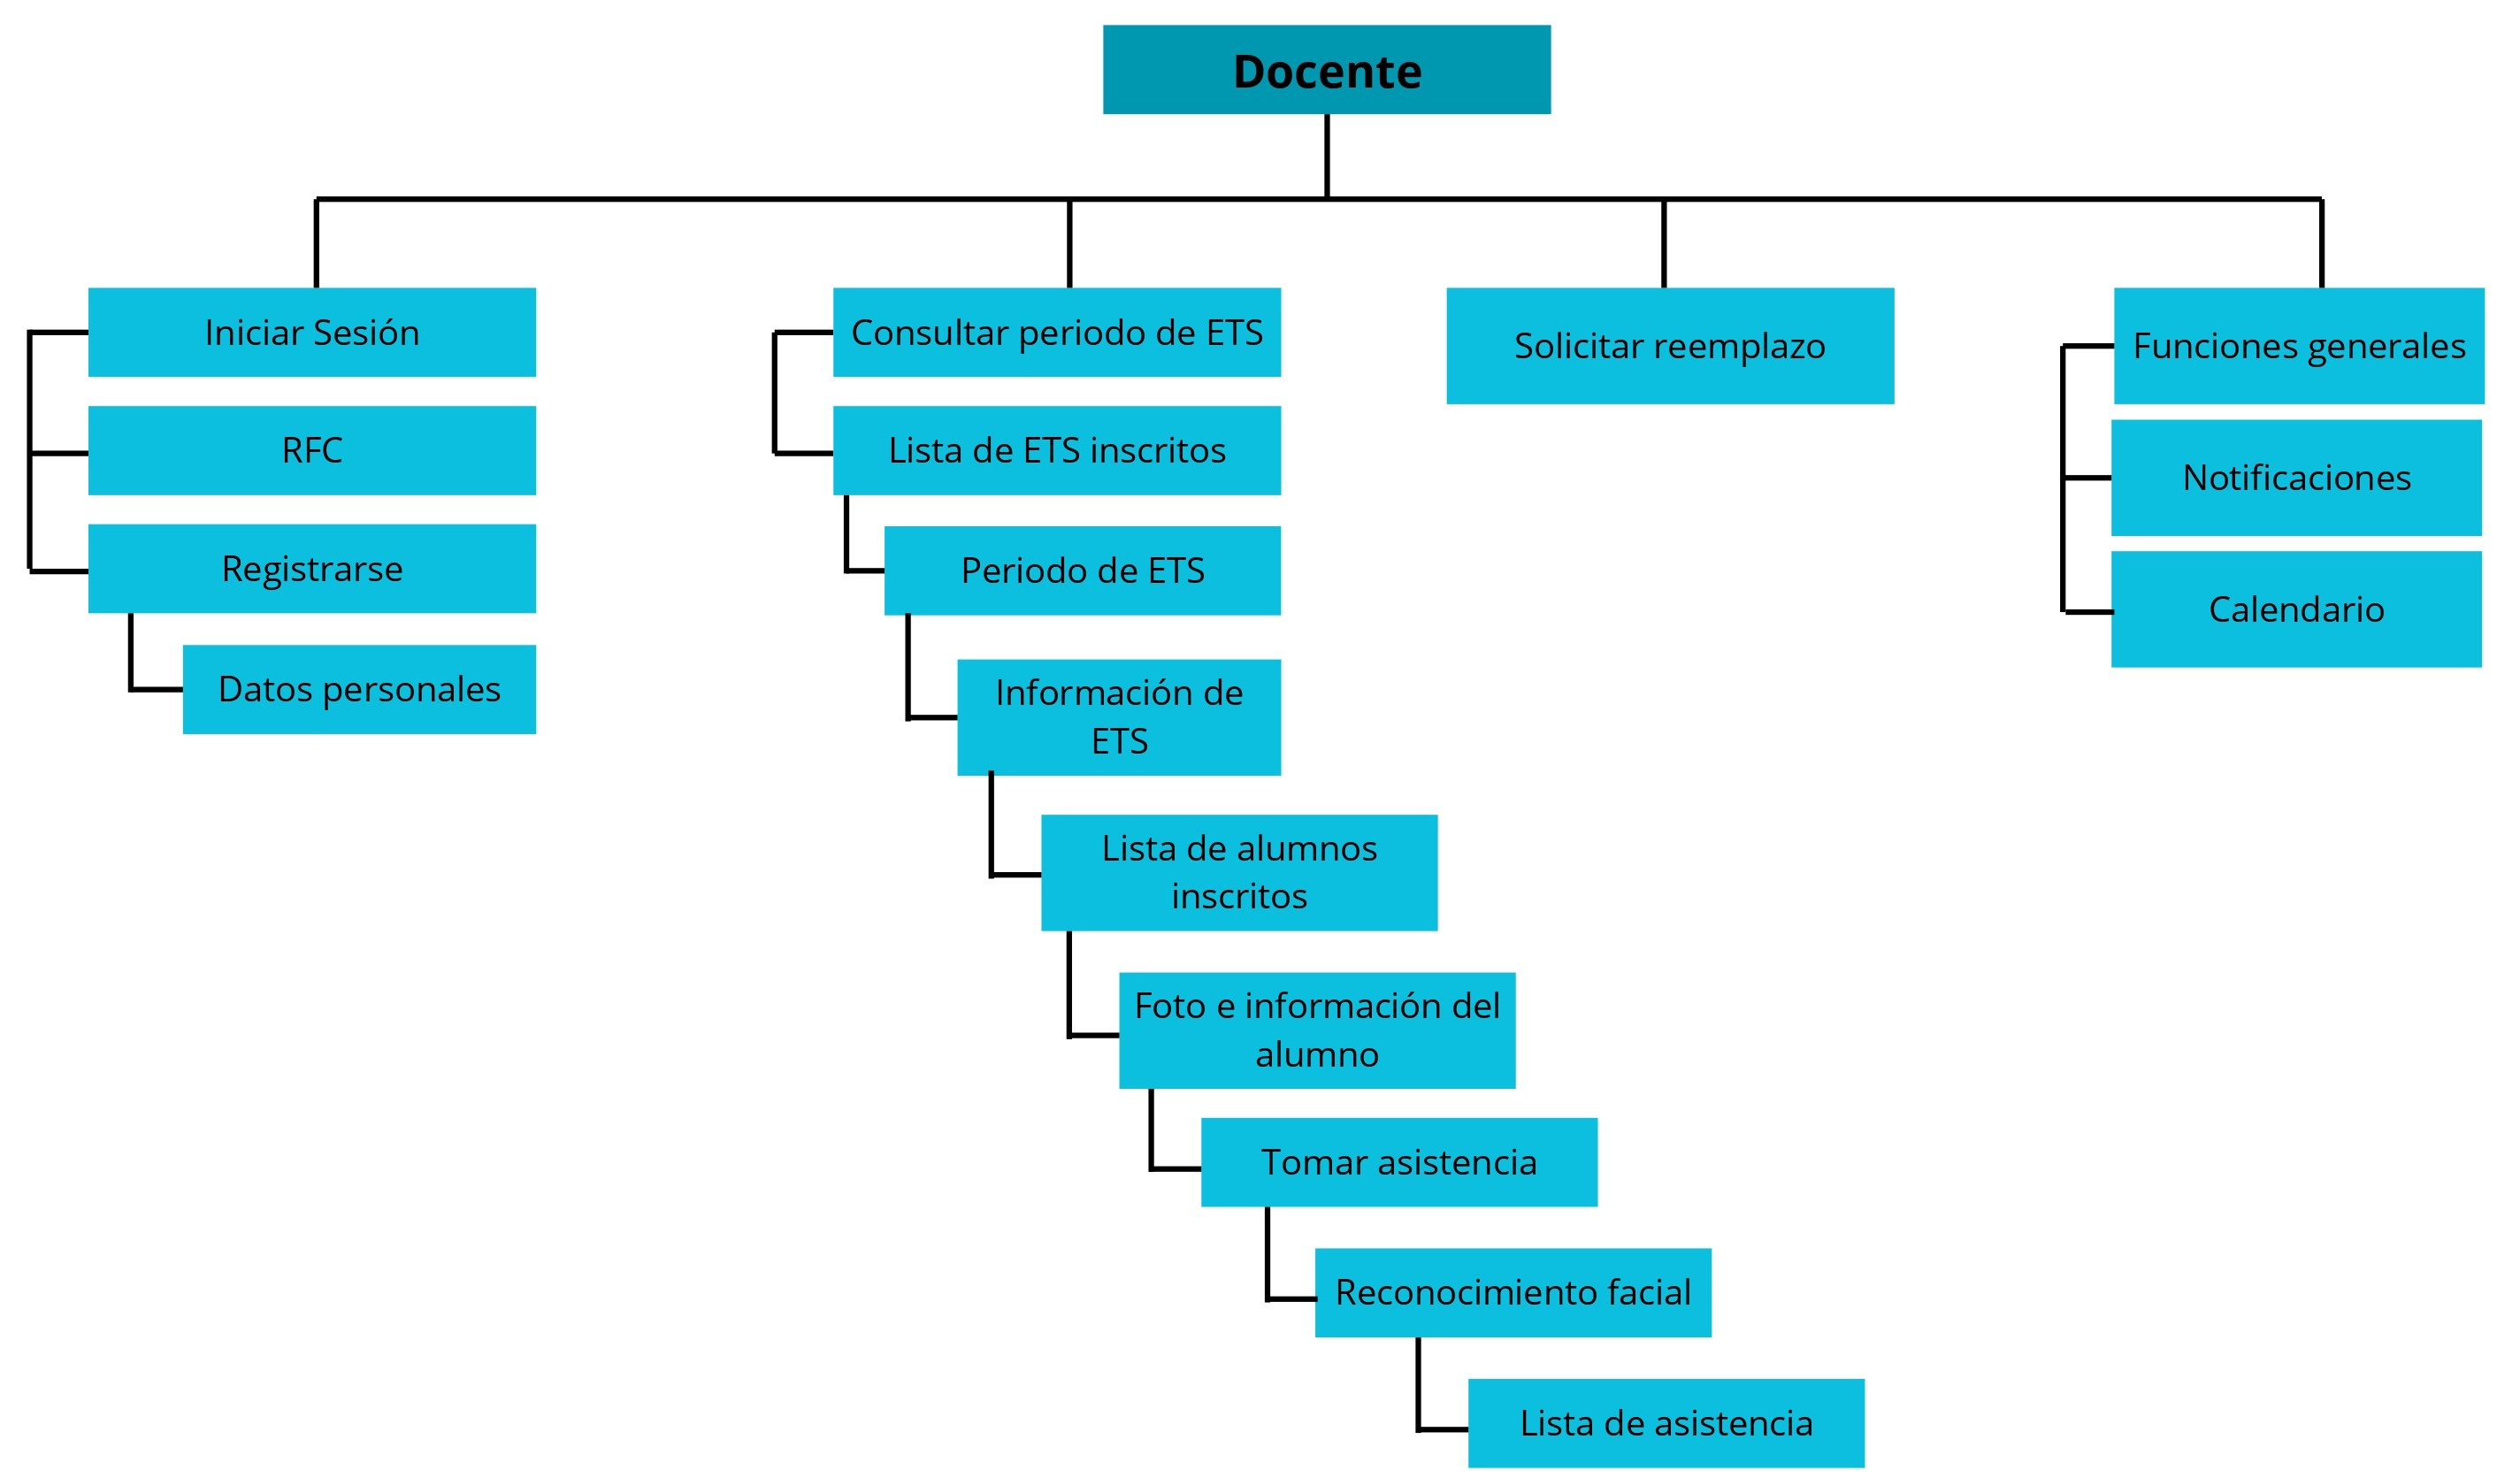
\includegraphics[width=1.0\textwidth]{images/docente}
		\caption{Mapa de navegación del docente}
		\label{fig:Mapa de navegación del docente}
	\end{center}
\end{figure}

\clearpage

\begin{figure}[htbp]
	\begin{center}
		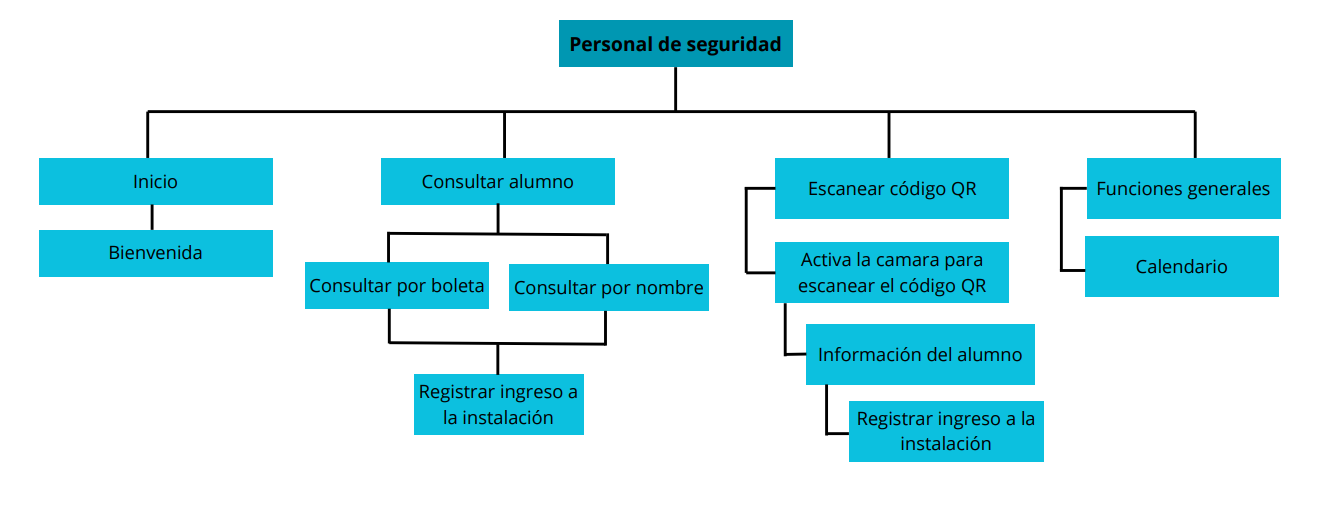
\includegraphics[width=.9\textwidth]{images/personalseguridad}
		\caption{Mapa de navegación del personal de seguridad}
		\label{fig:Mapa de navegación del personal de seguridad}
	\end{center}
\end{figure}

\newpage
% !TeX root = ../ejemplo.tex

%--------------------------------------
\subsection{IU01: Pantalla Iniciar sesión del sistema móvil}

\IUfig[.40]{UI-CU01}{IU01}{Pantalla Iniciar sesión del sistema móvil.}

\newpage

\subsubsection{Objetivo}
Controlar el acceso al sistema móvil, permitiendo a los usuarios registrados (docentes, personal de seguridad, alumnos, presidentes de academia y jefes de departamento) autenticarse mediante sus credenciales correspondientes.

\subsubsection{Diseño}
Esta pantalla \IUref{IU01}{Pantalla Iniciar sesión del sistema móvil} (ver figura~\ref{IU01}) es la primera que se muestra al iniciar la aplicación. Permite a los diferentes tipos de usuarios ingresar sus datos de autenticación.



La pantalla contiene los siguientes elementos:
\begin{itemize}
	\item \textbf{Título:} "Iniciar sesión".
	\item \textbf{Campo "Boleta":} Para que los alumnos ingresen su número de boleta. Tiene un icono de usuario asociado.
	\item \textbf{Campo "Contraseña":} Para que todos los usuarios ingresen su contraseña. Tiene un icono de candado asociado.
	\item \textbf{Botón \IUbutton{Entrar}:} Permite iniciar la sesión una vez que se han introducido las credenciales.
\end{itemize}

\subsubsection{Salidas}
Redirección a la pantalla de saludo correspondiente al rol del usuario autenticado, mostrando un saludo y su nombre. Las posibles pantallas de saludo son:
\begin{itemize}
	\item \IUref{IUE01}{Pantalla de saludo del docente} (para docentes, presidentes de academia y jefes de departamento).
	\item \IUref{IUE02}{Pantalla de saludo del personal de seguridad}.
	\item \IUref{IUE03}{Pantalla de saludo del alumno}.
	\item \IUref{IUE06}{Pantalla de saludo del presidente de academia/jefe de departamento} (también para presidentes de academia y jefes de departamento).
\end{itemize}

\subsubsection{Entradas}
Dependiendo del rol del usuario:
\begin{itemize}
	\item \textbf{Alumno:} Número de boleta y Contraseña.
	\item \textbf{Personal de seguridad:} CURP y Contraseña.
	\item \textbf{Docente, Presidente de academia, Jefe de departamento:} RFC y Contraseña.
\end{itemize}
	
	\subsubsection{Comandos}
	\begin{itemize}
		\item \IUbutton{Entrar}:
		\begin{enumerate}
			\item Verifica que se hayan llenado todos los campos (Boleta y Contraseña). Si falta algún campo, muestra el mensaje \textbf{\hyperref[msg:CU01-E1]{MSG-CU01-E1}}{``Por favor, completa todos los campos.''}.
			\item Verifica que las credenciales (Boleta y Contraseña) coincidan con un usuario registrado en el sistema. Si no coinciden, muestra el mensaje \textbf{\hyperref[msg:CU01-E2]{MSG-CU01-E2}} ``Datos incorrectos.''.
			\item En caso de pérdida de conexión durante la verificación, muestra el mensaje \textbf{\hyperref[msg:CU01-E3]{MSG-CU01-E3}} ``Conexión perdida.''.
			\item Si la autenticación es exitosa, determina el rol del usuario y lo redirige a la pantalla de saludo correspondiente (\IUref{IUE01}{Pantalla de saludo del docente}, \IUref{IUE02}{Pantalla de saludo del personal de seguridad}, \IUref{IUE03}{Pantalla de saludo del alumno} o \IUref{IUE06}{Pantalla de saludo del presidente de academia/jefe de departamento}).
		\end{enumerate}
		
	\end{itemize}
	
	\subsubsection{Mensajes}
	\begin{itemize}
		\item \textbf{\hyperref[msg:CU01-E1]{MSG-CU01-E1}} Por favor, completa todos los campos.
		\item \textbf{\hyperref[msg:CU01-E2]{MSG-CU01-E2}} Datos incorrectos.
		\item \textbf{\hyperref[msg:CU01-E3]{MSG-CU01-E3}} Conexión perdida.
	\end{itemize}



\newpage

% !TeX root = ../ejemplo2.tex

%--------------------------------------
\subsection{IU02: Pantalla Consultar calendario escolar}

\IUfig[.40]{UI-CU02}{IU02}{Pantalla Consultar calendario escolar.}

\newpage

\subsubsection{Objetivo}
Permitir a los usuarios visualizar el calendario escolar y obtener información sobre el tiempo restante para el inicio del próximo periodo de ETS.

\subsubsection{Diseño}
Esta pantalla \IUref{IU02}{Pantalla Consultar calendario escolar} (ver figura~\ref{IU02}) muestra el calendario escolar actual. Se puede acceder a ella mediante el botón con forma de calendario que está visible en la barra de navegación inferior, presente en la mayoría de las pantallas de la aplicación (excepto la de inicio de sesión).



La pantalla contiene los siguientes elementos:
\begin{itemize}
	\item \textbf{Barra de navegación superior:}
	\begin{itemize}
		\item \textbf{Icono de flecha hacia la izquierda:} Para regresar a la pantalla anterior.
		\item \textbf{Título:} Calendario Escolar.
		\item \textbf{Icono de tres puntos horizontales con una burbuja de diálogo:} Accede a la funcionalidad de mensajes dentro de la aplicación
	\end{itemize}
	\item \textbf{Imagen del Calendario Escolar:} Visualización del calendario académico actual.
	\item \textbf{Botón \IUbutton{Calcular cuántos días faltan para el periodo de ETS}:} Al presionarlo, el sistema calcula y muestra el tiempo restante para el próximo periodo de ETS.
	\item \textbf{Barra de navegación inferior:} Contiene iconos para:
	\begin{itemize}
		\item \textbf{Icono de casa:} Redirección a la pantalla de saludo correspondiente al usuario.
		\item \textbf{Icono de campana:} Redirección a la pantalla de notificaciones.
		\item \textbf{Icono de calendario con marcas:} Indica la pantalla actual del calendario.
		\item \textbf{Icono de flecha apuntando hacia la derecha saliendo de un recuadro:} Función de cerrar sesión.
	\end{itemize}
\end{itemize}

\subsubsection{Salidas}
Muestra un mensaje indicando cuántos días faltan para el periodo de ETS o si actualmente es periodo de ETS, en respuesta a la acción del botón \IUbutton{Calcular cuántos días faltan para el periodo de ETS}.

\subsubsection{Entradas}
Ninguna directa por parte del usuario en esta pantalla, más allá de la interacción con los botones.

\subsubsection{Comandos}
\begin{itemize}
	\item \IUbutton{Calcular cuántos días faltan para el periodo de ETS}:
	\begin{enumerate}
		\item Recupera la fecha de inicio del próximo periodo de ETS registrada en el sistema.
		\item Calcula la diferencia en días entre la fecha actual y la fecha de inicio del próximo periodo de ETS.
		\item Si la fecha de inicio es posterior a la actual, muestra el mensaje \textbf{ ``Faltan (cantidad de días) días para el periodo de ETS.''}
		\item Si la fecha de inicio es igual o anterior a la actual, muestra el mensaje \textbf{ ``Actualmente es periodo de ETS.''}
		\item En caso de que no se haya registrado el siguiente periodo de ETS, muestra el mensaje \textbf{ ``Aún no está registrado el siguiente periodo de ETS.''}
		\item En caso de pérdida de conexión, muestra el mensaje \textbf{ ``Conexión perdida.''}
	\end{enumerate}
	\item \textbf{Icono de campana (barra de navegación inferior):} Redirige a la pantalla \IUref{UI03}{Consultar notificaciones}.
	\item \textbf{Icono de casa (barra de navegación inferior):} Redirige a la pantalla de menú correspondiente al tipo de usuario.
	\item \textbf{Icono de flecha saliendo (barra de navegación inferior):} Función de cerrar sesión.
	\item \textbf{Icono de flecha izquierda (barra superior):} Regresa a la pantalla anterior.
	\item \textbf{Icono de tres puntos horizontales con una burbuja de diálogo:} Accede a la funcionalidad de mensajes dentro de la aplicación.
\end{itemize}

\subsubsection{Mensajes}

\begin{itemize}
	\item \textbf{ Faltan (cantidad de días) días para el periodo de ETS.}
	\item \textbf{ Actualmente es periodo de ETS.}
	\item \textbf{ Aún no está registrado el siguiente periodo de ETS.}
	\item \textbf{ Conexión perdida.}
\end{itemize}


\newpage

% !TeX root = ../ejemplo.tex

%--------------------------------------
\subsection{IU03 Pantalla Consultar notificaciones}

\subsubsection{Objetivo}
Permitir que los usuarios puedan gestionar sus notificaciones y marcarlas como leidas.
\subsubsection{Diseño}
    Esta pantalla \IUref{IU03}{Pantalla Consultar notificaciones } (ver figura~\ref{IU03}) puede ser accedida desde cualquier otra pantalla que no sea el inicio de sesión mediante el botón con forma de campana.
\IUfig[.35]{UI-CU03}{IU03}{Pantalla Consultar notificaciones.}

\subsubsection{Salidas}
Menciona que la notificación seleccionada ha sido establecida como leída.
\subsubsection{Entradas}
   Ninguna.

\subsubsection{Comandos}
\begin{itemize}
    \item \IUbutton{Botón con palomita} toma la notificación seleccionada y la marca como leída.
    \item \IUbutton{Buscador} En este buscador se puede buscar las notificaciones por fecha.
    \item \IUbutton{Calendario} Redirige a la pantalla \IUref{UI02}{Consultar calendario escolar}.
    \item \IUbutton{Home} Redirige a la pantalla de bienvenida correspondiente al tipo de usuario.
\end{itemize}

\subsubsection{Mensajes}
     
\begin{Citemize}
    \item {\bf MSG-8}{``Actualmente no hay notificaciones.}
\end{Citemize}



\newpage

%--------------------------------------
\subsection{IU04 Pantalla Periodo de ETS}

\subsubsection{Objetivo}
	Permitir al docente consultar los periodos de ETS que le han sido asignados. 

\subsubsection{Diseño}
	Esta pantalla \IUref{IU04}{Pantalla Periodo de ETS} (ver figura~\ref{IU04}) aparece luego de seleccionar la opción de Consultar Periodos de ETS de la pantalla principal. 

\IUfig[.35]{cu04}{IU04}{Pantalla Periodo de ETS.}

\subsubsection{Salidas}

	Lista de periodos de ETS asignados. 

\subsubsection{Entradas}
Ninguna

\subsubsection{Comandos}

\begin{Citemize}
	\item \IUbutton{Calendario} Redirige a la pantalla \IUref{UI02}{Consultar calendario escolar}.
	\item \IUbutton{Campana} Redirige a la pantalla \IUref{UI03}{Consultar notificaciones }.
	\item \IUbutton{Home} Redirige a la pantalla de bienvenida correspondiente al tipo de usuario.
	\item \IUbutton{Periodo de ETS} Selecciona un periodo de ETS y lo redirige a la \IUref{IU04}{pantalla Periodo de ETS}. 
\end{Citemize}


\subsubsection{Mensajes}

\begin{Citemize}
	\item {\bf MSG-9}{``Error al consultar la base de datos. Intente nuevamente más tarde''.}
	\item {\bf MSG-10}{``No tienes periodos de ETS asignados.''}
\end{Citemize}


\newpage

%--------------------------------------
\subsection{IU05 Pantalla Consultar ETS}

\subsubsection{Objetivo}
	Permitir al docente consultar los ETS que tiene asignados. 

\subsubsection{Diseño}
	Esta pantalla \IUref{IU05}{Pantalla Consultar ETS} (ver figura~\ref{IU05}) aparece luego de seleccionar un periodo de ETS. 

\IUfig[.35]{cu05}{IU05}{Pantalla Consultar ETS.}

\subsubsection{Salidas}
	Lista de ETS asignados. 

\subsubsection{Entradas}
	Ninguna
	
\subsubsection{Comandos}
\begin{Citemize}

	\item \IUbutton{Calendario} Redirige a la pantalla \IUref{UI02}{Consultar calendario escolar}.
	\item \IUbutton{Campana} Redirige a la pantalla \IUref{UI03}{Consultar notificaciones }.
	\item \IUbutton{Home} Redirige a la pantalla de bienvenida correspondiente al tipo de usuario.
	\item \IUbutton{ETS} Selecciona un ETS y lo redirige a la \IUref{IU06}{pantalla Información de ETS}.
\end{Citemize}

\subsubsection{Mensajes}

\begin{Citemize}
	\item {\bf MSG-9}{``Error al consultar la base de datos. Intente nuevamente más tarde.''.}
	\item {\bf MSG-11}{``No hay ETS asignados actualmente.''}
\end{Citemize}


\newpage

%--------------------------------------
\subsection{IU06: Pantalla Información de ETS}

\IUfig[.40]{cu06}{IU06}{Pantalla Información de ETS}
\newpage

\subsubsection{Objetivo}
Permitir al docente visualizar la información detallada cada ETS que tiene asignado.

\subsubsection{Diseño}
Esta pantalla \IUref{IU06}{Pantalla Información de ETS} (ver figura~\ref{IU06}) aparece luego de seleccionar un ETS asignado.



La pantalla contiene los siguientes elementos:
\begin{itemize}
	\item \textbf{Barra de navegación superior:}
	\begin{itemize}
		\item \textbf{Icono de flecha hacia la izquierda:} Para regresar a la pantalla anterior (\IUref{IU05}{Pantalla Consultar ETS}).
		\item \textbf{Título:} "Detalles del ETS de Bases de Datos".
		\item \textbf{Icono de tres puntos horizontales con una burbuja de diálogo:} Accede a la funcionalidad de mensajes dentro de la aplicación.
	\end{itemize}
	\item \textbf{Información del ETS:} Muestra los detalles del ETS en forma de lista o texto informativo:
	\begin{itemize}
		\item Unidad de aprendizaje.
		\item Tipo de ETS.
		\item Periodo.
		\item Fecha de aplicación.
		\item Turno.
		\item Duración.
		\item Salones asignados:
		\item Hora de inicio.
	\end{itemize}
	\item \textbf{Botón \IUbutton{Solicitar reemplazo}:} Visible si el docente es el aplicador del ETS. Redirige a la \IUref{IU07}{Pantalla Solicitar remplazo}.
	\item \textbf{Botón \IUbutton{Ir a la lista de alumnos}:} Visible si hay alumnos inscritos en el ETS. Redirige a la \IUref{IU08}{Pantalla Lista de alumnos inscritos a un ETS}.
	\item \textbf{Barra de navegación inferior:} Contiene iconos para:
	\begin{itemize}
		\item \textbf{Icono de casa:} Redirección a la pantalla de saludo correspondiente al tipo de usuario.
		\item \textbf{Icono de campana:} Redirección a la pantalla de notificaciones.
		\item \textbf{Icono de calendario con marcas:} Redirección a la pantalla \IUref{IU02}{Consultar calendario escolar}.
		\item \textbf{Icono de flecha apuntando hacia la derecha saliendo de un recuadro:} Cierra la sesión del usuario y lo regresa a la pantalla de inicio de sesión (\IUref{IU01}{Iniciar sesión del sistema móvil}).
	\end{itemize}
\end{itemize}

\subsubsection{Salidas}
Información detallada del ETS seleccionado.

\subsubsection{Entradas}
Ninguna

\subsubsection{Comandos}
\begin{itemize}
	\item \IUbutton{Solicitar reemplazo}: Redirige a la pantalla \IUref{IU07}{Solicitar remplazo}.
	\item \IUbutton{Ir a la lista de alumnos}: Redirige a la pantalla \IUref{IU08}{Lista de alumnos inscritos a un ETS}.
	\item \textbf{Icono de flecha izquierda (barra superior):} Regresa a la pantalla anterior (\IUref{IU05}{Pantalla Consultar ETS}).
	\item \textbf{Icono de tres puntos (barra superior):} Accede a la funcionalidad de mensajes dentro de la aplicación.
	\item \textbf{Icono de calendario (barra de navegación inferior):} Redirige a la pantalla \IUref{IU02}{Consultar calendario escolar}.
	\item \textbf{Icono de campana (barra de navegación inferior):} Redirige a la pantalla de notificaciones.
	\item \textbf{Icono de casa (barra de navegación inferior):} Redirección a la pantalla de saludo correspondiente al tipo de usuario.
	\item \textbf{Icono de flecha saliendo (barra de navegación inferior):} Cierra la sesión del usuario y lo regresa a la pantalla de inicio de sesión (\IUref{IU01}{Iniciar sesión del sistema móvil}).
\end{itemize}

\subsubsection{Mensajes}
\begin{itemize}
	\item \textbf{Ocurrió un error al desplegar los detalles del ETS.}
	\item \textbf{Error al consultar la base de datos. Intente nuevamente más tarde.}
\end{itemize}


\newpage

%--------------------------------------
\subsection{IU07: Pantalla de Solicitar remplazo}

\subsubsection{Objetivo}
Permitir al docente pedir que otro docente lo remplaze en la aplicacion de un ETS.

\subsubsection{Diseño}
Esta pantalla \IUref{IU07}{Pantalla de Solicitar remplazo} (ver figura~\ref{IU07}) aparece luego de que el docente presione el boton \IUbutton{Solicitar reemplazo} en la pantalla \IUref{IU06}{Pantalla Información de ETS}.

\IUfig[.35]{UI-CU43}{IU07}{Pantalla de Solicitar remplazo}

\subsubsection{Salidas}
Confirmación de envio de solicitud

\subsubsection{Entradas}
Identificador del ETS y razon por la que se pide el remplazo.

\subsubsection{Comandos}
\begin{itemize}
	\item \IUbutton{Enviar solicitud}: Permite enviar la notificación al jefe de departamento y/o al presidente de academia para pedir el remplazo.
	\item \IUbutton{Calendario} Redirige a la pantalla \IUref{UI02}{Consultar calendario escolar}.
    \item \IUbutton{Campana} Redirige a la pantalla \IUref{UI03}{Consultar notificaciones }.
    \item \IUbutton{Home} Redirige a la pantalla de bienvenida correspondiente al tipo de usuario.
\end{itemize}

\subsubsection{Mensajes}

\begin{itemize}
	\item \textbf{ ``Solicitud exitosa. La solicitud de reemplazo ha sido registrada correctamente''}
	\item \textbf{ ``Ya existe una solicitud pendiente para este ETS'', indicando que ya se ha realizado una solicitud previa para el ETS".}
\end{itemize}


\newpage

%--------------------------------------
\subsection{IU08: Pantalla Lista de asistencia de ETS}

\IUfig[.40]{cu08}{IU08}{Pantalla Lista de asistencia de ETS}
\newpage

\subsubsection{Objetivo}
Permitir al docente visualizar la lista de los alumnos inscritos en un ETS asignado, junto con su estado de asistencia, y acceder a las funciones de reporte dentro del periodo permitido.

\subsubsection{Diseño}
Esta pantalla \IUref{IU08}{Pantalla Lista de asistencia de ETS} (ver figura~\ref{IU08}) muestra la lista de alumnos inscritos en el ETS seleccionado. Se accede a ella al presionar el botón "Ir a la lista de alumnos"  desde la \IUref{IU06}{Pantalla Información de ETS}.



La pantalla contiene los siguientes elementos:
\begin{itemize}
	\item \textbf{Barra de navegación superior:}
	\begin{itemize}
		\item \textbf{Icono de flecha hacia la izquierda:} Para regresar a la pantalla anterior (\IUref{IU06}{Pantalla Información de ETS}).
		\item \textbf{Título:} ETS de Bases de Datos\newline 25/2\newline Lista de alumnos inscritos.
		\item \textbf{Icono de tres puntos horizontales con una burbuja de diálogo:} Accede a la funcionalidad de mensajes dentro de la aplicación.
	\end{itemize}
	\item \textbf{Lista de alumnos inscritos:} Muestra a los alumnos inscritos en el ETS en forma de tarjetas o filas. Para cada alumno se muestra:
	\begin{itemize}
		\item \textbf{Boleta y Nombre:} Presentados como texto. Este elemento, al ser presionado (si está habilitado), redirige a la \textbf{Pantalla Reporte} (\IUref{IUE07}{Creación del reporte}).
		\item \textbf{Icono de estado de asistencia:} Un icono visual que representa el estado de asistencia del alumno (ej., una "X" roja o una paloma verde). Al presionarlo, redirige a la \IUref{IU20}{Pantalla mostrar la foto e información del alumno} (solo dentro del periodo de tiempo especificado).
	\end{itemize}
	\item \textbf{Barra de navegación inferior:} Contiene iconos para:
	\begin{itemize}
		\item \textbf{Icono de casa:} Redirección a la pantalla de saludo correspondiente al tipo de usuario.
		\item \textbf{Icono de campana:} Redirección a la pantalla de notificaciones.
		\item \textbf{Icono de calendario con marcas:} Redirección a la pantalla \IUref{IU02}{Consultar calendario escolar}.
		\item \textbf{Icono de flecha apuntando hacia la derecha saliendo de un recuadro:} Cierra la sesión del usuario y lo regresa a la pantalla de inicio de sesión (\IUref{IU01}{Iniciar sesión del sistema móvil}).
	\end{itemize}
\end{itemize}

\subsubsection{Salidas}
Muestra la lista de los alumnos inscritos en el ETS, incluyendo su boleta, nombre y un icono de estado de asistencia. Puede mostrar mensajes informativos sobre el periodo de reporte y los permisos del docente.

\subsubsection{Entradas}
Ninguna directa por parte del usuario en esta pantalla, ya que la lista se muestra al acceder a ella.

\subsubsection{Comandos}
\begin{itemize}
	\item \textbf{Boleta y Nombre del alumno (al ser presionado):} Si está habilitado (dentro del periodo de reporte y si el docente tiene permisos), redirige a la \textbf{Pantalla Reporte} (\IUref{IUE07}{Creación del reporte}).
	\item \textbf{Icono de estado de asistencia (al ser presionado):} Redirige a la \IUref{IU20}{Pantalla mostrar la foto e información del alumno} (solo dentro del periodo de tiempo especificado).
	\item \textbf{Icono de calendario (barra de navegación inferior):} Redirige a la pantalla \IUref{IU02}{Consultar calendario escolar}.
	\item \textbf{Icono de campana (barra de navegación inferior):} Redirige a la pantalla de notificaciones.
	\item \textbf{Icono de casa (barra de navegación inferior):} Redirección a la pantalla de saludo correspondiente al tipo de usuario.
	\item \textbf{Icono de flecha saliendo (barra de navegación inferior):} Cierra la sesión del usuario y lo regresa a la pantalla de inicio de sesión (\IUref{IU01}{Iniciar sesión del sistema móvil}).
	\item \textbf{Icono de flecha izquierda (barra superior):} Regresa a la pantalla anterior (\IUref{IU06}{Pantalla Información de ETS}).
	\item \textbf{Icono de tres puntos (barra superior):} Accede a la funcionalidad de mensajes dentro de la aplicación.
\end{itemize}

\subsubsection{Mensajes}
\begin{itemize}
	\item \textbf{\hyperref[msg:CU08-E2]{MSG-CU08-E2}} Error al consultar la base de datos. Intente nuevamente más tarde.
	\item \textbf{\hyperref[msg:CU08-A1]{MSG-CU08-A1}} No hay alumnos inscritos al ETS.
	\item \textbf{\hyperref[msg:CU08-C1]{MSG-CU08-C1}} El ETS seleccionado no es válido.
	\item \textbf{\hyperref[msg:CU08-D1]{MSG-CU08-D1}} Aún no es periodo para crear los reportes. Faltan (tiempo).
	\item \textbf{\hyperref[msg:CU08-ET2]{MSG-CU08-ET2}} El periodo para registrar los reportes ha concluido.
	\item \textbf{\hyperref[msg:CU08-F1]{MSG-CU08-F1}} Usted no está autorizado para crear el reporte de este alumno.
\end{itemize}
\newpage

%--------------------------------------
\subsection{IU09 Asignar docente de remplazo}

\subsubsection{Objetivo}
Permitir al jefe de departamento y/o al presidente de academia responder a las solicitudes de remplazo y asignar un docente de remplazo para el ETS especifico.

\subsubsection{Diseño}
Esta pantalla \IUref{IU09}{Asignar docente de remplazo} (ver figura~\ref{IU09}) aparece luego de que el jefe de departamento y/o al presidente de academia revisen sus notificaciones y seleccione una solicitud de remplazo.

\IUfig[.35]{UI-CU44}{IU09}{Pantalla de Asignar docente de remplazo}

\subsubsection{Salidas}
Confirmación de asignación del nuevo docente y se muestra el mensaje {\bf MSG-42}{``docente de remplazo asignado con exito.''}.

\subsubsection{Entradas}
Identificador del ETS y nombre del nuevo docente asignado.

\subsubsection{Comandos}
\begin{itemize}
	\item \IUbutton{Asignar}: Permite enviar la notificación docente de que su remplzado ha sido asignado y ademas asigna el remplazo como docente aplicador en el sistema.
\end{itemize}

\subsubsection{Mensajes}

\begin{Citemize}
	\item {\bf MSG-28} {``El proceso no se pudo realizar por un fallo de red''.}
	\item {\bf MSG-42}{``docente de remplazo asignado con exito'.'}
\end{Citemize}



\newpage


%--------------------------------------
\subsection{IU10 Pantalla Código QR}

\subsubsection{Objetivo}
Permitir al personal de seguridad escanear el código QR de la credencial del alumno.

\subsubsection{Diseño}
Esta pantalla \IUref{IU10}{Pantalla Código QR} (ver figura~\ref{IU10}) aparece una vez que el personal de seguridad inicia sesión. 

\IUfig[.35]{cu12}{IU10}{Pantalla Código QR}

\subsubsection{Salidas}
Información del alumno

\subsubsection{Entradas}
Ninguna

\subsubsection{Comandos}
\begin{itemize}
	\item \IUbutton{Escanear}: Permite escanear el código QR de la credencial del alumno.
	\item \IUbutton{Calendario} Redirige a la pantalla \IUref{UI02}{Consultar calendario escolar}.
    \item \IUbutton{Campana} Redirige a la pantalla \IUref{UI03}{Consultar notificaciones }.
    \item \IUbutton{Home} Redirige a la pantalla de bienvenida correspondiente al tipo de usuario.
\end{itemize}

\subsubsection{Mensajes}
Ninguno


\newpage

%--------------------------------------
\subsection{IU11 Pantalla Credencial del alumno}

\subsubsection{Objetivo}
	Permitir al personal de seguridad consultar la información del alumno mediante el escaneo del código QR de su credencial.

\subsubsection{Diseño}
Esta pantalla aparece luego de que se escanea el código QR de la credencial del alumno \IUref{IU11}{Pantalla Credencial del alumno} (ver figura~\ref{IU11}).
	

\IUfig[.35]{cu14}{IU11}{Pantalla Credencial del alumno}

\subsubsection{Salidas}
	Información del alumno

\subsubsection{Entradas}
Ninguna

\subsubsection{Comandos}
\begin{itemize}
	\item \IUbutton{Registrar asistencia}: Permite registrar la asistencia del alumno.
	\item \IUbutton{Calendario} Redirige a la pantalla \IUref{UI02}{Consultar calendario escolar}.
    \item \IUbutton{Campana} Redirige a la pantalla \IUref{UI03}{Consultar notificaciones }.
    \item \IUbutton{Home} Redirige a la pantalla de bienvenida correspondiente al tipo de usuario.
\end{itemize}

\subsubsection{Mensajes}

\begin{Citemize}
	\item {\bf MSG-20}{``Alumno no registrado''}
	\item {\bf MSG-11}{``Error al consultar la base de datos. Intente nuevamente más tarde.''}
\end{Citemize}


\newpage

%--------------------------------------
\subsection{IU12 Pantalla Buscar alumno}

\subsubsection{Objetivo}
    Permitir al personal de seguridad buscar la información de un alumno utilizando su número de boleta o su nombre. 

\subsubsection{Diseño}
    Esta pantalla \IUref{IU12}{Pantalla Buscar alumno} (ver figura~\ref{IU12}) aparece luego de seleccionar la opción Consultar alumno. 

\IUfig[.35]{cu13}{IU12}{Pantalla Buscar alumno por boleta.}

\subsubsection{Salidas}
    Información del alumno.

\subsubsection{Entradas}
    Número de boleta del alumno o su nombre. 

\subsubsection{Comandos}
\begin{itemize}
    \item Buscador por boleta: Permite al personal de seguridad buscar al alumno ingresando su número de boleta.
    \item Buscador por boleta: Permite al personal de seguridad buscar al alumno ingresando su nombre.
    \item \IUbutton{Calendario} Redirige a la pantalla \IUref{UI02}{Consultar calendario escolar}.
    \item \IUbutton{Campana} Redirige a la pantalla \IUref{UI03}{Consultar notificaciones }.
    \item \IUbutton{Home} Redirige a la pantalla de bienvenida correspondiente al tipo de usuario.
\end{itemize}

\subsubsection{Mensajes}

\begin{Citemize}
    \item {\bf MSG-21}{``número de boleta ingresado no corresponde a ningún alumno registrado''}
    \item {\bf MSG-9}{``Error al consultar la base de datos. Intente nuevamente más tarde.''}
    \item {\bf MSG-22}{``Alumno no registrado''}
\end{Citemize}



\newpage

%%--------------------------------------
\subsection{IU12-2 Pantalla Buscar alumno por nombre}

\subsubsection{Objetivo}
Permitir al personal de seguridad buscar la información de un alumno utilizando su nombre. 

\subsubsection{Diseño}
Esta pantalla \IUref{IU12}{Pantalla Buscar alumno} aparece luego de seleccionar la opción Consultar alumno. 

\IUfig[.35]{cu11}{IU12}{Pantalla Buscar alumno.}

\subsubsection{Salidas}
Información del alumno.

\subsubsection{Entradas}
Nombre del alumno. 

\subsubsection{Comandos}

\begin{itemize}

	\item Buscador: Permite al usuario buscar al alumno ingresando su nombre. 
	\item \IUbutton{Calendario} Redirige a la pantalla \IUref{UI02}{Consultar calendario escolar}.
    \item \IUbutton{Campana} Redirige a la pantalla \IUref{UI03}{Consultar notificaciones }.
    \item \IUbutton{Home} Redirige a la pantalla de bienvenida correspondiente al tipo de usuario.
\end{itemize}

\subsubsection{Mensajes}

\begin{Citemize}
	\item {\bf MSG-20}{``Alumno no registrado''}
\end{Citemize}



%\newpage

%--------------------------------------
\subsection{IU13: Pantalla consultar lista de alumnos inscritos a un ETS}

\subsubsection{Objetivo}
Permitir al docente visualizar la lista de los alumnos inscritos a un ETS asignado.

\subsubsection{Diseño}
Esta pantalla aparece luego de seleccionar un ETS en la \IUref{IU13}{Pantalla Informacion de ETS} (ver figura~\ref{IU06} y muestra la boleta, el nombre completo y la foto de los alumnos inscritos al ETS)

\IUfig[.35]{cu07}{IU13}{Consultar lista de alumnos inscritos a un ETS}

\subsubsection{Salidas}
Lista de los alumnos inscritos al ETS.

\subsubsection{Entradas}
Ninguna

\subsubsection{Comandos}
\begin{itemize}
    \item \IUbutton{Calendario} Redirige a la pantalla \IUref{UI02}{Consultar calendario escolar}.
    \item \IUbutton{Campana} Redirige a la pantalla \IUref{UI03}{Consultar notificaciones }.
    \item \IUbutton{Home} Redirige a la pantalla de bienvenida correspondiente al tipo de usuario.
	\item \IUbutton{Tomar asistencia} redirige a la pantalla \IUref{IU08}{Lista de asistencia de ETS}.
\end{itemize}

\subsubsection{Mensajes}

\begin{Citemize}
	\item {\bf MSG-14}{``No hay alumnos inscritos en este ETS.''}
	\item {\bf MSG9-}{``Error al consultar la base de datos. Intente nuevamente más tarde.''}. 
\end{Citemize}
\newpage

%--------------------------------------
\subsection{IU14: Pantalla Periodo de ETS del alumno}

\subsubsection{Objetivo}
	Permitir al alumno consultar los periodos de ETS que le han sido asignados. 

\subsubsection{Diseño}
	Esta pantalla \IUref{IU14}{Pantalla Periodo de ETS del alumno} (ver figura~\ref{IU14}) aparece luego de seleccionar la opción de Consultar Periodos.

\IUfig[.35]{cu16}{IU14}{Pantalla Periodo de ETS del alumno.}

\subsubsection{Salidas}
	Lista de periodos de ETS. 

\subsubsection{Entradas}
Ninguna

\subsubsection{Comandos}

\begin{itemize}
	\item \IUbutton{Calendario} Redirige a la pantalla \IUref{UI02}{Consultar calendario escolar}.
	\item \IUbutton{Campana} Redirige a la pantalla \IUref{UI03}{Consultar notificaciones }.
	\item \IUbutton{Home} Redirige a la pantalla de bienvenida correspondiente al tipo de usuario.
	\item \IUbutton{Periodo de ETS} Selecciona un periodo de ETS y lo redirige a la pantalla \IUref{UI15}{consultar ETS del alumno}.
\end{itemize}

\subsubsection{Mensajes}

\begin{Citemize}
	\item {\bf MSG-25}{``No hay periodos de ETS''}
	\item {\bf MSG-9}{``Error al consultar la base de datos. Intente nuevamente más tarde.''}
\end{Citemize}


\newpage

%--------------------------------------
\subsection{IU15: Pantalla Consultar ETS del alumno}

\IUfig[.35]{cu17}{IU15}{Pantalla Consultar ETS del alumno.}
\label{IU15}
\newpage

\subsubsection{Objetivo}
Permitir al alumno visualizar la lista de los ETS en los que se ha inscrito y, opcionalmente, filtrarlos por nombre.

\subsubsection{Diseño}
Esta pantalla \IUref{IU15}{Pantalla Consultar ETS del alumno} (ver figura~\ref{IU15}) aparece luego de que el alumno selecciona el botón \IUbutton{Listado de ETS} en la \IUref{IUE03}{Pantalla de saludo del alumno}.

La pantalla contiene los siguientes elementos:
\begin{itemize}
	\item \textbf{Barra de navegación superior:}
	\begin{itemize}
		\item \textbf{Icono de flecha hacia la izquierda:} Para regresar a la pantalla anterior (\IUref{IUE03}{Pantalla de saludo del alumno}).
		\item \textbf{Título:} "Lista de ETS".
		\item \textbf{Icono de tres puntos horizontales con una burbuja de diálogo:} Accede a la funcionalidad de mensajes dentro de la aplicación.
	\end{itemize}
	\item \textbf{Barra de búsqueda:} Campo de texto donde el alumno puede ingresar el nombre de un ETS para filtrar la lista.
	\begin{itemize}
		\item \textbf{Botón \IUbutton{Todos}:} Muestra todos los ETS.
		\item \textbf{Botón \IUbutton{Mis ETS}:} Muestra los ETS en los que el alumno está inscrito.
	\end{itemize}
	\item \textbf{Lista de ETS inscritos:} Muestra una lista de los ETS en los que el alumno se ha inscrito. Por cada ETS muestra:
	\begin{itemize}
		\item Unidad de Aprendizaje.
		\item Periodo.
		\item Fecha.
		\item Turno.
	\end{itemize}
	Al seleccionar un elemento de esta lista, se navega a la \IUref{IU16}{Pantalla Información de ETS del alumno}.
	\item \textbf{Barra de navegación inferior:} Contiene iconos para:
	\begin{itemize}
		\item \textbf{Icono de casa:} Redirección a la pantalla de saludo del alumno (\IUref{IUE03}{Pantalla de saludo del alumno}).
		\item \textbf{Icono de campana:} Redirección a la pantalla de notificaciones.
		\item \textbf{Icono de calendario con marcas:} Redirección a la pantalla \IUref{IU02}{Consultar calendario escolar}.
		\item \textbf{Icono de flecha apuntando hacia la derecha saliendo de un recuadro:} Cierra la sesión del usuario y lo regresa a la pantalla de inicio de sesión (\IUref{IU01}{Iniciar sesión del sistema móvil}).
	\end{itemize}
\end{itemize}

\subsubsection{Salidas}
Lista de ETS inscritos (con nombre, periodo, fecha, turno) o indicación de que no hay ETS inscritos.

\subsubsection{Entradas}
Término de búsqueda ingresado por el alumno. Selección de un ETS de la lista. Selección de los botones de filtro.

\subsubsection{Comandos}
\begin{itemize}
	\item \textbf{Ingresar texto en la barra de búsqueda:} Filtra la lista de ETS por nombre.
	\item \textbf{Seleccionar un ETS de la lista:} Navega a la \IUref{IU16}{Pantalla Información de ETS del alumno}.
	\item \textbf{Botón \IUbutton{Todos}:} Muestra todos los ETS inscritos.
	\item \textbf{Botón \IUbutton{Mis ETS}:} Muestra los ETS inscritos del alumno.
	\item \textbf{Icono de flecha izquierda (barra superior):} Regresa a la pantalla anterior (\IUref{IUE03}{Pantalla de saludo del alumno}).
	\item \textbf{Icono de tres puntos (barra superior):} Accede a la funcionalidad de mensajes dentro de la aplicación.
	\item \textbf{Icono de calendario (barra de navegación inferior):} Redirige a la pantalla \IUref{IU02}{Consultar calendario escolar}.
	\item \textbf{Icono de campana (barra de navegación inferior):} Redirige a la pantalla de notificaciones.
	\item \textbf{Icono de casa (barra de navegación inferior):} Redirección a la pantalla de saludo del alumno (\IUref{IUE03}{Pantalla de saludo del alumno}).
	\item \textbf{Icono de flecha saliendo (barra de navegación inferior):} Cierra la sesión del usuario y lo regresa a la pantalla de inicio de sesión (\IUref{IU01}{Iniciar sesión del sistema móvil}).
\end{itemize}

\subsubsection{Mensajes}
\begin{itemize}
	\item \textbf{Error al consultar la base de datos. Intente nuevamente más tarde.}
	\item \textbf{Conexión perdida.}
	\item \textbf{No hay ETS inscritos.}
\end{itemize}

\newpage

%%--------------------------------------
\subsection{IU15: Pantalla Consultar ETS del alumno}

\IUfig[.35]{cu17}{IU15}{Pantalla Consultar ETS del alumno.}
\label{IU15}
\newpage

\subsubsection{Objetivo}
Permitir al alumno visualizar la lista de los ETS en los que se ha inscrito y, opcionalmente, filtrarlos por nombre.

\subsubsection{Diseño}
Esta pantalla \IUref{IU15}{Pantalla Consultar ETS del alumno} (ver figura~\ref{IU15}) aparece luego de que el alumno selecciona el botón \IUbutton{Listado de ETS} en la \IUref{IUE03}{Pantalla de saludo del alumno}.

La pantalla contiene los siguientes elementos:
\begin{itemize}
	\item \textbf{Barra de navegación superior:}
	\begin{itemize}
		\item \textbf{Icono de flecha hacia la izquierda:} Para regresar a la pantalla anterior (\IUref{IUE03}{Pantalla de saludo del alumno}).
		\item \textbf{Título:} "Lista de ETS".
		\item \textbf{Icono de tres puntos horizontales con una burbuja de diálogo:} Accede a la funcionalidad de mensajes dentro de la aplicación.
	\end{itemize}
	\item \textbf{Barra de búsqueda:} Campo de texto donde el alumno puede ingresar el nombre de un ETS para filtrar la lista.
	\begin{itemize}
		\item \textbf{Botón \IUbutton{Todos}:} Muestra todos los ETS.
		\item \textbf{Botón \IUbutton{Mis ETS}:} Muestra los ETS en los que el alumno está inscrito.
	\end{itemize}
	\item \textbf{Lista de ETS inscritos:} Muestra una lista de los ETS en los que el alumno se ha inscrito. Por cada ETS muestra:
	\begin{itemize}
		\item Unidad de Aprendizaje.
		\item Periodo.
		\item Fecha.
		\item Turno.
	\end{itemize}
	Al seleccionar un elemento de esta lista, se navega a la \IUref{IU16}{Pantalla Información de ETS del alumno}.
	\item \textbf{Barra de navegación inferior:} Contiene iconos para:
	\begin{itemize}
		\item \textbf{Icono de casa:} Redirección a la pantalla de saludo del alumno (\IUref{IUE03}{Pantalla de saludo del alumno}).
		\item \textbf{Icono de campana:} Redirección a la pantalla de notificaciones.
		\item \textbf{Icono de calendario con marcas:} Redirección a la pantalla \IUref{IU02}{Consultar calendario escolar}.
		\item \textbf{Icono de flecha apuntando hacia la derecha saliendo de un recuadro:} Cierra la sesión del usuario y lo regresa a la pantalla de inicio de sesión (\IUref{IU01}{Iniciar sesión del sistema móvil}).
	\end{itemize}
\end{itemize}

\subsubsection{Salidas}
Lista de ETS inscritos (con nombre, periodo, fecha, turno) o indicación de que no hay ETS inscritos.

\subsubsection{Entradas}
Término de búsqueda ingresado por el alumno. Selección de un ETS de la lista. Selección de los botones de filtro.

\subsubsection{Comandos}
\begin{itemize}
	\item \textbf{Ingresar texto en la barra de búsqueda:} Filtra la lista de ETS por nombre.
	\item \textbf{Seleccionar un ETS de la lista:} Navega a la \IUref{IU16}{Pantalla Información de ETS del alumno}.
	\item \textbf{Botón \IUbutton{Todos}:} Muestra todos los ETS inscritos.
	\item \textbf{Botón \IUbutton{Mis ETS}:} Muestra los ETS inscritos del alumno.
	\item \textbf{Icono de flecha izquierda (barra superior):} Regresa a la pantalla anterior (\IUref{IUE03}{Pantalla de saludo del alumno}).
	\item \textbf{Icono de tres puntos (barra superior):} Accede a la funcionalidad de mensajes dentro de la aplicación.
	\item \textbf{Icono de calendario (barra de navegación inferior):} Redirige a la pantalla \IUref{IU02}{Consultar calendario escolar}.
	\item \textbf{Icono de campana (barra de navegación inferior):} Redirige a la pantalla de notificaciones.
	\item \textbf{Icono de casa (barra de navegación inferior):} Redirección a la pantalla de saludo del alumno (\IUref{IUE03}{Pantalla de saludo del alumno}).
	\item \textbf{Icono de flecha saliendo (barra de navegación inferior):} Cierra la sesión del usuario y lo regresa a la pantalla de inicio de sesión (\IUref{IU01}{Iniciar sesión del sistema móvil}).
\end{itemize}

\subsubsection{Mensajes}
\begin{itemize}
	\item \textbf{Error al consultar la base de datos. Intente nuevamente más tarde.}
	\item \textbf{Conexión perdida.}
	\item \textbf{No hay ETS inscritos.}
\end{itemize}

%--------------------------------------
\subsection{IU16 Pantalla Información de ETS}

\subsubsection{Objetivo}
Permitir al alumno visualizar la información detallada cada ETS que tiene inscrito.

\subsubsection{Diseño}
Esta pantalla \IUref{IU16}{Pantalla de Información de ETS del alumno} (ver figura~\ref{IU16}) aparece luego de seleccionar un ETS inscrito. 

\IUfig[.35]{cu18}{IU16}{Pantalla de Información de ETS del alumno}

\subsubsection{Salidas}

Información detallada del ETS seleccionado. 

\subsubsection{Entradas}
Ninguna


\subsubsection{Comandos}
\begin{itemize}
	\item \IUbutton{Calendario} Redirige a la pantalla \IUref{UI02}{Consultar calendario escolar}.
    \item \IUbutton{Campana} Redirige a la pantalla \IUref{UI03}{Consultar notificaciones }.
    \item \IUbutton{Home} Redirige a la pantalla de bienvenida correspondiente al tipo de usuario.
\end{itemize}

\subsubsection{Mensajes}

\begin{Citemize}
	\item {\bf MSG-13}{``Información no disponible para el ETS seleccinado''}
	\item {\bf MSG-11}{``Error al consultar la base de datos. Intente nuevamente más tarde.''}
\end{Citemize}



\newpage

%--------------------------------------
\subsection{IU17 Pantalla de Reconocimiento facial}

\subsubsection{Objetivo}
Permitir al docente registrar la asistencia al ETS de los alumnos y al personal de seguridad le permite registrar la entrada a las instalaciones.

\subsubsection{Diseño}
Esta pantalla \IUref{IU17}{Pantalla de Reconocimiento facial} (ver figura~\ref{IU17}) aparece luego de seleccionar el botón \IUbutton{Registrar asistencia} desde la pantalla \IUref{IU08}{Lista de asistencia de ETS}..


\IUfig[.30]{cu19}{IU17}{Pantalla de Reconocimiento facial}

\subsubsection{Salidas}
Confirmación de asistencia registrada

\subsubsection{Entradas}
Ninguna

\subsubsection{Comandos}
\begin{itemize}
    \item \IUbutton{Cancelar}: Permite al alumno cancelar la operación de Reconocimeinto facial.
    \item \IUbutton{Comenzar}: Activa la cámara para el Reconocimiento facil. 
    \item \IUbutton{Calendario} Redirige a la pantalla \IUref{UI02}{Consultar calendario escolar}.
    \item \IUbutton{Campana} Redirige a la pantalla \IUref{UI03}{Consultar notificaciones }.
    \item \IUbutton{Home} Redirige a la pantalla de bienvenida correspondiente al tipo de usuario.
    \item \IUbutton{Registrar asistencia} Si el usuario que presiona el botón es un docente, marca la asistencia del alumno al ETS, por otro lado si el usuario que presiona es un botón personal de seguridad, marca la entrada del alumno a las instalaciones.
    \item \IUbutton{No registrar asistencia} No marca la asistencia ni la entrada (El alumno no es quien dice ser).
\end{itemize}

\subsubsection{Mensajes}

\begin{Citemize}
    \item {\bf MSG-17}{``No se pudo activar la cámara o reconocer la identidad. Intente nuevamente.''}
    \item {\bf MSG-16}{``No hay alumnos inscritos en este ETS.''}
    \item {\bf MSG-9}{``Error al consultar la base de datos. Intente nuevamente más tarde.''}
    \item {\bf MSG-15}{``Asistencia registrada exitosamente.''}
    \item {\bf MSG-23}{``Entrada registrada exitosamente.''}
    \item {\bf MSG-24}{``Entrada no registrada .''}
\end{Citemize}

\newpage

%--------------------------------------
\subsection{IU18: Pantalla de Detalles del proceso de ETS}

\IUfig[.35]{CU20}{IU18}{Pantalla de Detalles del proceso de ETS}
\label{IU18}
\newpage

\subsubsection{Objetivo}
Permitir al alumno visualizar la información detallada sobre los pasos a seguir para la inscripción al ETS.

\subsubsection{Diseño}
Esta pantalla \IUref{IU18}{Pantalla de Detalles del proceso de ETS} (ver figura~\ref{IU18}) aparece luego de seleccionar el botón \IUbutton{Información de Acceso} en la \IUref{IUE03}{Pantalla saludo del alumno}.

La pantalla contiene los siguientes elementos:
\begin{itemize}
	\item \textbf{Barra de navegación superior:}
	\begin{itemize}
		\item \textbf{Icono de flecha hacia la izquierda:} Para regresar a la pantalla anterior (\IUref{IUE03}{Pantalla saludo del alumno}).
		\item \textbf{Título:} "Guía de Inscripción al ETS".
		\item \textbf{Icono de tres puntos horizontales con una burbuja de diálogo:} Accede a la funcionalidad de mensajes dentro de la aplicación.
	\end{itemize}
	\item \textbf{Lista de pasos para la inscripción al ETS:} Muestra los pasos numerados para la inscripción, cada uno dentro de un recuadro con un fondo claro:
	\begin{itemize}
		\item \textbf{1.} Pagar en caja y verificar que estén correctos los siguientes datos: Nombre, Boleta, Carrera y Número de unidades de aprendizaje.
		\item \textbf{2.} Acudir a ventanilla de gestión escolar para generar créditos en el "SAES".
		\item \textbf{3.} Una vez generados los créditos, inscribir las unidades de aprendizaje en la página del "SAES".
		\item \textbf{4.} Entregar en ventanilla de gestión escolar el comprobante de inscripción de ETS generado por SAES y el recibo de pago para finalizar la inscripción al ETS.
		\item \textbf{5.} Acudir el día y la hora establecida en el calendario.
	\end{itemize}
	\item \textbf{Barra de navegación inferior:} Contiene iconos para:
	\begin{itemize}
		\item \textbf{Icono de casa:} Redirección a la (\IUref{IUE03}{Pantalla de saludo del alumno}.
		\item \textbf{Icono de campana:} Redirección a la pantalla de notificaciones.
		\item \textbf{Icono de calendario con marcas:} Redirección a la pantalla \IUref{IU02}{Consultar calendario escolar}.
		\item \textbf{Icono de flecha apuntando hacia la derecha saliendo de un recuadro:} Cierra la sesión del usuario y lo regresa a la pantalla de inicio de sesión (\IUref{IU01}{Iniciar sesión del sistema móvil}).
	\end{itemize}
\end{itemize}

\subsubsection{Salidas}
Información detallada de los pasos para la inscripción al ETS.

\subsubsection{Entradas}
Ninguna.

\subsubsection{Comandos}
\begin{itemize}
	\item \textbf{Icono de flecha izquierda (barra superior):} Regresa a la pantalla anterior (\IUref{IUE03}{Pantalla saludo del alumno}).
	\item \textbf{Icono de tres puntos (barra superior):} Accede a la funcionalidad de mensajes dentro de la aplicación.
	\item \textbf{Icono de calendario (barra de navegación inferior):} Redirige a la pantalla \IUref{IU02}{Consultar calendario escolar}.
	\item \textbf{Icono de campana (barra de navegación inferior):} Redirige a la pantalla de notificaciones.
	\item \textbf{Icono de casa (barra de navegación inferior):} Redirección a la pantalla de saludo correspondiente al tipo de usuario.
	\item \textbf{Icono de flecha saliendo (barra de navegación inferior):} Cierra la sesión del usuario y lo regresa a la pantalla de inicio de sesión (\IUref{IU01}{Iniciar sesión del sistema móvil}).
\end{itemize}

\subsubsection{Mensajes}
\begin{itemize}
	\item \textbf{Error al recuperar la información del proceso. Intente nuevamente más tarde.}
\end{itemize}


\newpage

\subsection{IU19: Pantalla de Reconocimiento facial alumno}

\IUfig[.40]{cu19-2}{IU19}{Pantalla de Reconocimiento facial alumno.}
\newpage	

\subsubsection{Objetivo}
Permitir al alumno probar la funcionalidad de reconocimiento facial.

\subsubsection{Diseño}
Esta pantalla \IUref{IU19}{Pantalla de Reconocimiento facial alumno} (ver figura~\ref{IU19}) aparece al seleccionar el botón "Probar reconocimiento facial" en la pantalla \IUref{IU16}{Pantalla de Información de ETS del alumno}. Su diseño es similar a la \IUref{IU17}{Pantalla de Reconocimiento facial} (ver figura~\ref{IU17}).



La pantalla contiene los siguientes elementos:
\begin{itemize}
	\item \textbf{Barra de navegación superior:}
	\begin{itemize}
		\item \textbf{Icono de flecha hacia la izquierda:} Para regresar a la pantalla anterior (\IUref{IUE07}{Pantalla Crear Reporte}).
		\item \textbf{Título:} "Tome la fotografía".
		\item \textbf{Icono de tres puntos horizontales con una burbuja de diálogo:} Accede a la funcionalidad de mensajes dentro de la aplicación.
	\end{itemize}
	\item \textbf{Vista de la cámara:} Un área central oscura que muestra la vista previa de lo que la cámara del dispositivo está enfocando, indicando dónde debe colocarse el rostro del alumno para tomar la fotografía. Un recuadro.
	\item \textbf{Botón de captura:} Un círculo con un icono de cámara en el centro, ubicado en la parte inferior central de la pantalla. Al presionarlo, se toma la fotografía del alumno.
	\item \textbf{Barra de navegación inferior:} Contiene iconos para:
	\begin{itemize}
		\item \textbf{Icono de casa:} Redirección a la pantalla de saludo correspondiente al tipo de usuario.
		\item \textbf{Icono de campana:} Redirección a la pantalla de notificaciones.
		\item \textbf{Icono de calendario con marcas:} Redirección a la pantalla \IUref{IU02}{Consultar calendario escolar}.
		\item \textbf{Icono de flecha apuntando hacia la derecha saliendo de un recuadro:} Cierra la sesión del usuario y lo regresa a la pantalla de inicio de sesión (\IUref{IU01}{Iniciar sesión del sistema móvil}).
	\end{itemize}
\end{itemize}

\subsubsection{Salidas}
Después de tomar la fotografía, el sistema procesa la imagen para el reconocimiento facial y regresa a la \IUref{IUE03}{Saludo del alumno}, mostrando una confirmación de que el reconocimiento facial funciona (o un mensaje de error si falla).

\subsubsection{Entradas}
La fotografía capturada por la cámara del dispositivo al presionar el botón de captura.

\subsubsection{Comandos}
\begin{itemize}
	\item \textbf{Botón de captura (icono de cámara):} Activa la toma de la fotografía.
	\item \textbf{Icono de flecha izquierda (barra superior):} Regresa a la pantalla anterior.
	\item \textbf{Icono de tres puntos (barra superior):} Accede a la funcionalidad de mensajes dentro de la aplicación.
	\item \textbf{Icono de calendario (barra de navegación inferior):} Redirige a la pantalla \IUref{IU02}{Consultar calendario escolar}.
	\item \textbf{Icono de campana (barra de navegación inferior):} Redirige a la pantalla de notificaciones.
	\item \textbf{Icono de casa (barra de navegación inferior):} Redirección a la pantalla de saludo correspondiente al tipo de usuario.
	\item \textbf{Icono de flecha saliendo (barra de navegación inferior):} Cierra la sesión del usuario y lo regresa a la pantalla de inicio de sesión (\IUref{IU01}{Iniciar sesión del sistema móvil}).
\end{itemize}

\subsubsection{Mensajes}
\begin{itemize}
	\item \textbf{Error al capturar la fotografía: [detalle del error].}
	\item \textbf{Error al realizar el reconocimiento facial: [detalle del error].}
	\item \textbf{Error de conexión. (Podría ocurrir durante el proceso de reconocimiento).}
	\item \textbf{Ocurrió un fallo en el proceso. (Un error general durante el reconocimiento).}
\end{itemize}
\newpage

%--------------------------------------
\subsection{IU20: Mostrar la foto e información del alumno}

\IUfig[.40]{cu11}{IU20}{Mostrar la foto e información del alumno.}

\newpage

\subsubsection{Objetivo}
Mostrar al docente la información detallada del alumno seleccionado y los elementos multimedia asociados a su registro de asistencia en el ETS.

\subsubsection{Diseño}
Esta pantalla \IUref{IU20}{Pantalla Reporte del Alumno} (ver figura~\ref{IU20}) se muestra al seleccionar un alumno desde la \IUref{IU08}{Pantalla Lista de asistencia de ETS}. Presenta información del alumno y elementos relacionados con su asistencia.



La pantalla contiene los siguientes elementos:
\begin{itemize}
	\item \textbf{Barra de navegación superior:}
	\begin{itemize}
		\item \textbf{Icono de flecha hacia la izquierda:} Para regresar a la pantalla anterior (\IUref{IU08}{Pantalla Lista de asistencia de ETS}).
		\item \textbf{Título:} Reporte.
		\item \textbf{Icono de tres puntos horizontales con una burbuja de diálogo:} Accede a la funcionalidad de mensajes dentro de la aplicación.
	\end{itemize}
	\item \textbf{Información del Alumno y Reporte de Asistencia:} Muestra la siguiente información (si está disponible):
	\begin{itemize}
		\item \textbf{Foto de la credencial:} Imagen del documento de identificación del alumno. Si no se carga, se muestra el texto "Sin Imagen".
		\item \textbf{Foto del reconocimiento facial:} Imagen capturada durante el proceso de reconocimiento facial, junto con la precisión del reconocimiento. Si no hubo verificación facial, esta información no se muestra.
		\item \textbf{Boleta:} Número de boleta del alumno.
		\item \textbf{Nombre completo:} Nombre completo del alumno.
		\item \textbf{CURP:} Clave Única de Registro de Población del alumno.
		\item \textbf{Carrera:} Programa académico que cursa el alumno.
		\item \textbf{Unidad académica del ETS:} Escuela o facultad a la que pertenece el ETS.
		\item \textbf{Periodo del ETS:} Periodo académico en el que se imparte el ETS.
		\item \textbf{Turno del ETS:} Turno en el que se aplica el ETS.
		\item \textbf{Materia del ETS:} Nombre de la unidad de aprendizaje del ETS.
		\item \textbf{Tipo de ETS:} Modalidad del Examen Terminal (ej., Ordinario).
		\item \textbf{Fecha de ingreso:} Fecha de ingreso del alumno al sistema (o al ETS, según el contexto).
		\item \textbf{Hora de ingreso:} Hora en la que se registró la asistencia del alumno (si aplica).
		\item \textbf{Nombre del docente aplicador:} Nombre del docente que aplicó el ETS.
		\item \textbf{Razón del reporte:} Justificación o comentarios sobre la asistencia del alumno.
		\item \textbf{Motivo del rechazo:} Si la asistencia fue rechazada, se muestra la razón.
	\end{itemize}
	\item \textbf{Barra de navegación inferior:} Contiene iconos para:
	\begin{itemize}
		\item \textbf{Icono de casa:} Redirección a la pantalla de saludo correspondiente al tipo de usuario.
		\item \textbf{Icono de campana:} Redirección a la pantalla de notificaciones.
		\item \textbf{Icono de calendario con marcas:} Redirección a la pantalla \IUref{IU02}{Consultar calendario escolar}.
		\item \textbf{Icono de flecha apuntando hacia la derecha saliendo de un recuadro:} Cierra la sesión del usuario y lo regresa a la pantalla de inicio de sesión (\IUref{IU01}{Iniciar sesión del sistema móvil}).
	\end{itemize}
\end{itemize}

\subsubsection{Salidas}
Muestra la información detallada del alumno y su reporte de asistencia, incluyendo los elementos mencionados en el diseño (si están disponibles).

\subsubsection{Entradas}
Ninguna directa por parte del usuario en esta pantalla, ya que la información se muestra al seleccionar un alumno en la pantalla anterior.

\subsubsection{Comandos}
\begin{itemize}
	\item \IUbutton{Ampliar fotografía}: Muestra la fotografía del alumno ampliada.
	\item \textbf{Icono de flecha izquierda (barra superior):} Regresa a la pantalla anterior (\IUref{IU08}{Pantalla Lista de asistencia de ETS}).
	\item \textbf{Icono de tres puntos (barra superior):} Accede a la funcionalidad de mensajes dentro de la aplicación.
	\item \textbf{Icono de calendario (barra de navegación inferior):} Redirección a la pantalla \IUref{IU02}{Consultar calendario escolar}.
	\item \textbf{Icono de campana (barra de navegación inferior):} Redirección a la pantalla de notificaciones.
	\item \textbf{Icono de casa (barra de navegación inferior):} Redirección a la pantalla de saludo correspondiente al tipo de usuario.
	\item \textbf{Icono de flecha saliendo (barra de navegación inferior):} Cierra la sesión del usuario y lo regresa a la pantalla de inicio de sesión (\IUref{IU01}{Iniciar sesión del sistema móvil}).
\end{itemize}

\subsubsection{Mensajes}
\begin{itemize}
	\item \textbf{\hyperref[msg:CU11-E1]{MSG-CU11-E1}} El proceso no se pudo realizar por un fallo de red.
	\item \textbf{\hyperref[msg:CU11-A1]{MSG-CU11-A1}} No se ha creado reporte para este alumno.
	\item \textbf{\hyperref[msg:CU11-B1]{MSG-CU11-B1}} El alumno no se presentó al ETS.
\end{itemize}

\newpage

% !TeX root = ../ejemplo.tex

%--------------------------------------
\subsection{IU21 Dar de alta a alumno}

\subsubsection{Objetivo}
	Permitir al personal de la DAE dar de alta a un alumno.
\subsubsection{Diseño}
    Esta pantalla \IUref{IU21}{ Dar de alta a alumno } (ver figura~\ref{IU21}) puede ser accedida desde la pantalla \IUref{IUE04}{de personal de la DAE}

\IUfig[1]{UI-CU21}{IU21}{ Dar de alta a alumno.}

\subsubsection{Salidas}
Muestra mensaje {\bf MSG-31} ``Alumno dado de alta con éxito''.
\subsubsection{Entradas}
    Boleta, Nombre, CURP, Sexo y Correo institucional
\subsubsection{Comandos}
\begin{itemize}
    \item \IUbutton{Dar de alta un alumno}  El sistema revisa que los datos del alumno sean válidos, verifica que el CURP o la boleta no hayan sido registrados con anterioridad, mantiene los datos para usarlos en el proceso de crear credencial. Y redirige a la pantalla \IUref{UI22}{Crear credencial}.
    \item \IUbutton{Home} Redirige a la pantalla de bienvenida correspondiente al tipo de usuario.
    
\end{itemize}

\subsubsection{Mensajes}

\begin{Citemize}
    \item {\bf MSG-31} ``Alumno dado de alta con éxito''.
    \item {\bf MSG-28}  ``El proceso no se pudo realizar por un falló de red.''
    \item {\bf MSG-29}{``Los campos no están correctamente llenados.''}
    \item {\bf MSG-30}{``La CURP o la boleta ya han sido asociadas a este alumno con anterioridad u otro alumno.''}
\end{Citemize}

\newpage

% !TeX root = ../ejemplo.tex

%--------------------------------------
\subsection{IU22: Crear credencial}

\subsubsection{Objetivo}
   Permite al personal de gestión escolar revisar una previsualización de la credencial del alumno y revisar los datos.
\subsubsection{Diseño}
    Esta pantalla \IUref{IU22}{ Crear credencial } (ver figura~\ref{IU22}) puede ser accedida desde la pantalla \IUref{IU21}{ Dar de alta a alumno} apretando el botón \IUbutton{Dar de alta alumno }.

\IUfig[1]{UI-CU22}{IU22}{ Crear credencial.}

\subsubsection{Salidas}
Ninguna
\subsubsection{Entradas}
    Boleta, Nombre, CURP, Sexo y Correo institucional
\subsubsection{Comandos}
\begin{itemize}
\item \IUbutton{Subir foto} Guarda la información y redirige a la pantalla \IUref{UI23}{ Capturar fotografía estudiantil }.
    \item \IUbutton{Home} Redirige a la pantalla de bienvenida correspondiente al tipo de usuario.
    
\end{itemize}

\subsubsection{Mensajes}

\begin{Citemize}
    \item {\bf  ``El proceso no se pudo realizar por un falló de red.''}
    \item {\bf``Los campos no están correctamente llenados.''}
    \item {\bf``El CURP o la boleta ya han sido asociadas a este alumno con anterioridad u otro alumno.''}
\end{Citemize}

\newpage

%--------------------------------------
\subsection{IU20: Mostrar la foto e información del alumno}

\IUfig[.40]{cu11}{IU20}{Mostrar la foto e información del alumno.}

\newpage

\subsubsection{Objetivo}
Mostrar al docente la información detallada del alumno seleccionado y los elementos multimedia asociados a su registro de asistencia en el ETS.

\subsubsection{Diseño}
Esta pantalla \IUref{IU20}{Pantalla Reporte del Alumno} (ver figura~\ref{IU20}) se muestra al seleccionar un alumno desde la \IUref{IU08}{Pantalla Lista de asistencia de ETS}. Presenta información del alumno y elementos relacionados con su asistencia.



La pantalla contiene los siguientes elementos:
\begin{itemize}
	\item \textbf{Barra de navegación superior:}
	\begin{itemize}
		\item \textbf{Icono de flecha hacia la izquierda:} Para regresar a la pantalla anterior (\IUref{IU08}{Pantalla Lista de asistencia de ETS}).
		\item \textbf{Título:} Reporte.
		\item \textbf{Icono de tres puntos horizontales con una burbuja de diálogo:} Accede a la funcionalidad de mensajes dentro de la aplicación.
	\end{itemize}
	\item \textbf{Información del Alumno y Reporte de Asistencia:} Muestra la siguiente información (si está disponible):
	\begin{itemize}
		\item \textbf{Foto de la credencial:} Imagen del documento de identificación del alumno. Si no se carga, se muestra el texto "Sin Imagen".
		\item \textbf{Foto del reconocimiento facial:} Imagen capturada durante el proceso de reconocimiento facial, junto con la precisión del reconocimiento. Si no hubo verificación facial, esta información no se muestra.
		\item \textbf{Boleta:} Número de boleta del alumno.
		\item \textbf{Nombre completo:} Nombre completo del alumno.
		\item \textbf{CURP:} Clave Única de Registro de Población del alumno.
		\item \textbf{Carrera:} Programa académico que cursa el alumno.
		\item \textbf{Unidad académica del ETS:} Escuela o facultad a la que pertenece el ETS.
		\item \textbf{Periodo del ETS:} Periodo académico en el que se imparte el ETS.
		\item \textbf{Turno del ETS:} Turno en el que se aplica el ETS.
		\item \textbf{Materia del ETS:} Nombre de la unidad de aprendizaje del ETS.
		\item \textbf{Tipo de ETS:} Modalidad del Examen Terminal (ej., Ordinario).
		\item \textbf{Fecha de ingreso:} Fecha de ingreso del alumno al sistema (o al ETS, según el contexto).
		\item \textbf{Hora de ingreso:} Hora en la que se registró la asistencia del alumno (si aplica).
		\item \textbf{Nombre del docente aplicador:} Nombre del docente que aplicó el ETS.
		\item \textbf{Razón del reporte:} Justificación o comentarios sobre la asistencia del alumno.
		\item \textbf{Motivo del rechazo:} Si la asistencia fue rechazada, se muestra la razón.
	\end{itemize}
	\item \textbf{Barra de navegación inferior:} Contiene iconos para:
	\begin{itemize}
		\item \textbf{Icono de casa:} Redirección a la pantalla de saludo correspondiente al tipo de usuario.
		\item \textbf{Icono de campana:} Redirección a la pantalla de notificaciones.
		\item \textbf{Icono de calendario con marcas:} Redirección a la pantalla \IUref{IU02}{Consultar calendario escolar}.
		\item \textbf{Icono de flecha apuntando hacia la derecha saliendo de un recuadro:} Cierra la sesión del usuario y lo regresa a la pantalla de inicio de sesión (\IUref{IU01}{Iniciar sesión del sistema móvil}).
	\end{itemize}
\end{itemize}

\subsubsection{Salidas}
Muestra la información detallada del alumno y su reporte de asistencia, incluyendo los elementos mencionados en el diseño (si están disponibles).

\subsubsection{Entradas}
Ninguna directa por parte del usuario en esta pantalla, ya que la información se muestra al seleccionar un alumno en la pantalla anterior.

\subsubsection{Comandos}
\begin{itemize}
	\item \IUbutton{Ampliar fotografía}: Muestra la fotografía del alumno ampliada.
	\item \textbf{Icono de flecha izquierda (barra superior):} Regresa a la pantalla anterior (\IUref{IU08}{Pantalla Lista de asistencia de ETS}).
	\item \textbf{Icono de tres puntos (barra superior):} Accede a la funcionalidad de mensajes dentro de la aplicación.
	\item \textbf{Icono de calendario (barra de navegación inferior):} Redirección a la pantalla \IUref{IU02}{Consultar calendario escolar}.
	\item \textbf{Icono de campana (barra de navegación inferior):} Redirección a la pantalla de notificaciones.
	\item \textbf{Icono de casa (barra de navegación inferior):} Redirección a la pantalla de saludo correspondiente al tipo de usuario.
	\item \textbf{Icono de flecha saliendo (barra de navegación inferior):} Cierra la sesión del usuario y lo regresa a la pantalla de inicio de sesión (\IUref{IU01}{Iniciar sesión del sistema móvil}).
\end{itemize}

\subsubsection{Mensajes}
\begin{itemize}
	\item \textbf{\hyperref[msg:CU11-E1]{MSG-CU11-E1}} El proceso no se pudo realizar por un fallo de red.
	\item \textbf{\hyperref[msg:CU11-A1]{MSG-CU11-A1}} No se ha creado reporte para este alumno.
	\item \textbf{\hyperref[msg:CU11-B1]{MSG-CU11-B1}} El alumno no se presentó al ETS.
\end{itemize}

\newpage

% !TeX root = ../ejemplo.tex

%--------------------------------------
\subsection{IU23: Capturar fotografía estudiantil}

\subsubsection{Objetivo}
   Permite agregar una foto a la credencial, para su posterior registro, además de obtener 5 fotos para ser guardadas en la base de datos.
\subsubsection{Diseño}
    Esta pantalla \IUref{IU23}{ Capturar fotografía estudiantil} (ver figura~\ref{IU23}) puede ser accedida desde la pantalla \IUref{IU22}{ Crear credencial} apretando el botón \IUbutton{Subir foto}

\IUfig[1]{UI-CU23}{IU23}{ Capturar fotografía estudiantil.}

\subsubsection{Salidas}
Ninguna
\subsubsection{Entradas}
Ninguna
\subsubsection{Comandos}
\begin{itemize}
    \item \IUbutton{Cámara} Toma 5 fotos al alumno, las cuales guarda en la base de datos para el sistema de reconocimiento facial, de estas la primera la usa para la credencial y redirige a la pantalla \IUref{UI21}{ Capturar fotografía estudiantil }.
    \item \IUbutton{Home} Redirige a la pantalla de bienvenida correspondiente al tipo de usuario.
    
\end{itemize}

\subsubsection{Mensajes}

\begin{Citemize}
    \item {\bf  ``El proceso no se pudo realizar por un fallo de red.''}
\end{Citemize}


\newpage

% !TeX root = ../ejemplo.tex

%--------------------------------------
\subsection{IU24 Consultar lista de periodo de ETS}
\subsubsection{Objetivo}
   Permite al personal de gestión escolar consultar una lista con todos los periodos de ETS y el periodo de ETS más actual en la parte superior.
\subsubsection{Diseño}
    Esta pantalla \IUref{IU24}{ Consultar lista de periodo de ETS } (ver figura~\ref{IU24}) puede ser accedida desde la pantalla \IUref{IUE05}{de saludo de gestión escolar } apretando el botón \IUbutton{Consultar lista de periodo de ETS}
\IUfig[1]{UI-CU24}{IU24}{ Consultar lista de periodo de ETS.}

\subsubsection{Salidas}
Ninguna
\subsubsection{Entradas}
Ninguna
\subsubsection{Comandos}
\begin{itemize}
    \item \IUbutton{ Dar de alta periodo de ETS } Redirige a la pantalla \IUref{UI25}{ Dar de alta de periodo de ETS}.
    \item \IUbutton{Home} Redirige a la pantalla de bienvenida correspondiente al tipo de usuario.
    
\end{itemize}

\subsubsection{Mensajes}

\begin{Citemize}
    \item {\bf MSG-28}  ``El proceso no se pudo realizar por un fallo de red.''
    \item {\bf MSG-31}  ``Ningún periodo de ETS ha sido dado de alta.''
\end{Citemize}



\newpage

% !TeX root = ../ejemplo.tex

%--------------------------------------
\subsection{IU25: Dar de alta periodo de ETS}
\subsubsection{Objetivo}
    Permite al personal de gestión escolar dar de alta un periodo de ETS.
\subsubsection{Diseño}
    Esta pantalla \IUref{IU25}{Dar de alta periodo de ETS } (ver figura~\ref{IU25}) puede ser accedida presionando el botón \IUbutton{Dar de alta periodo} desde el menú lateral, el cual estará disponible desde cualquier pantalla. 
    
\IUfig[1]{UI-CU25}{IU25}{Dar de alta un periodo de ETS.}

\subsubsection{Salidas}
Muestra mensaje {\bf ``Periodo de ETS  dado de alta con éxito''.}
\subsubsection{Entradas}
Periodo, Tipo de periodo, Fecha de inicio y Fecha de fin
\subsubsection{Comandos}
\begin{itemize}
	\item \IUbutton{Inicio}: Redirige al personal de gestion escolar a la pantalla \IUref{IUE05}{Pantalla inicial de personal de gestión escolar}
	
	\item \IUbutton{Dar de alta periodo}: Redirige al personal de gestión escolar a la pantalla \IUref{IU25}{Dar de alta periodo de ETS}
	\item \IUbutton{Consultar periodos}: Redirige al personal de gestión escolar a la pantalla \IUref{IU24}{Consultar lista de periodo de ETS}
	
	\item \IUbutton{Dar de alta ETS}: Redirige al personal de gestión escolar a la pantalla \IUref{IU27}{Dar de alta ETS}
	\item \IUbutton{Consultar lista de ETS}: Redirige al personal de gestión escolar a la pantalla \IUref{IU26}{Consultar lista de ETS}
	
	\item \IUbutton{Dar de alta docentes}: Redirige al personal de gestión escolar a la pantalla \IUref{IU31}{Dar de alta docente}
	\item \IUbutton{Consultar lista de docentes}: Redirige al personal de gestión escolar a la pantalla \IUref{IU30}{Consultar lista de docentes}
	
	\item \IUbutton{Dar de alta p. seguridad}: Redirige al personal de gestión escolar a la pantalla \IUref{IU29}{Dar de alta personal de seguridad}
	\item \IUbutton{Consultar lista de p. seguridad}: Redirige al personal de gestión escolar a la pantalla \IUref{IU28}{Consultar lista de personal de seguridad}
	
    \item \IUbutton{Guardar} Da de alta el nuevo periodo de ETS.
    
\end{itemize}

\subsubsection{Mensajes}

\begin{Citemize}
    \item {\bf ``Periodo de ETS  dado de alta con éxito''.}
    \item {\bf ``Los campos no están correctamente llenados.''}
    \item {\bf `` Periodo, Fecha de inicio o Fecha de fin ya han sido asociadas a un periodo de ETS.''}
\end{Citemize}


\newpage

% !TeX root = ../ejemplo.tex

%--------------------------------------
\subsection{IU26 Consultar lista de ETS}
\subsubsection{Objetivo}
    Permite al personal de gestión escolar consultar una lista con todos ETS.
\subsubsection{Diseño}
    Esta pantalla \IUref{IU26}{Consultar lista de ETS} (ver figura~\ref{IU26}) puede ser accedida desde la pantalla \IUref{IUE05}{ de saludo de gestión escolar } apretando el botón \IUbutton{Consultar lista de ETS}
\IUfig[]{UI-CU28}{IU26}{Consultar lista ETS.}

\subsubsection{Salidas}
Ninguna
\subsubsection{Entradas}
Ninguna
\subsubsection{Comandos}
\begin{itemize}
    \item \IUbutton{Dar de alta un ETS} Redirige a la pantalla \IUref{UI27}{ Dar de alta ETS}.
    \item \IUbutton{Home} Redirige a la pantalla de bienvenida correspondiente al tipo de usuario.
    
\end{itemize}

\subsubsection{Mensajes}

\begin{Citemize}
    \item {\bf MSG-28}  ``El proceso no se pudo realizar por un fallo de red.''
    \item {\bf MSG-34}  ``Ningún ETS ha sido dado da alta.''
\end{Citemize}


\newpage

% !TeX root = ../ejemplo.tex

%--------------------------------------
\subsection{IU27 Dar de alta ETS}
\subsubsection{Objetivo}
    Permite al personal de gestión escolar dar de alta un ETS.
\subsubsection{Diseño}
    Esta pantalla \IUref{IU27}{Dar de alta ETS} (ver figura~\ref{IU27}) puede ser accedida desde la pantalla \IUref{IU26}{Consultar lista de ETS} apretando el botón \IUbutton{Dar de alta un ETS}
\IUfig[1]{UI-CU29}{IU27}{Dar de alta ETS.}

\subsubsection{Salidas}
Muestra mensaje {\bf MSG-35} ``ETS  dado de alta con éxito''.
\subsubsection{Entradas}
ETS, Periodo-de-ETS, Fecha, Turno, Cupo , Unidad-de-aprendizaje,  Salon y Docente.
\subsubsection{Comandos}
\begin{itemize}
    \item \IUbutton{Dar de alta ETS} Da de alta el nuevo ETS y redirige a la pantalla \IUref{UI26}{Consultar lista de ETS}.
    \item \IUbutton{Home} Redirige a la pantalla de bienvenida correspondiente al tipo de usuario.
    
\end{itemize}

\subsubsection{Mensajes}

\begin{Citemize}
    \item {\bf MSG-35} ``ETS  dado de alta con éxito''.
    \item {\bf MSG-28}  ``El proceso no se pudo realizar por un fallo de red.''
    \item {\bf MSG-29}{``Los campos no están correctamente llenados.''}
    \item {\bf MSG-36}{`` ETS o salón  ya han sido asociadas a un ETS de ETS.''}
    
\end{Citemize}


\newpage

% !TeX root = ../ejemplo.tex

%--------------------------------------
\subsection{IU28: Consultar lista de personal de seguridad}
\subsubsection{Objetivo}
   Permite al personal de gestión escolar consultar una lista con todo el personal de seguridad.
\subsubsection{Diseño}
    Esta pantalla \IUref{IU28}{Consultar lista de personal de seguridad} (ver figura~\ref{IU28}) puede ser accedida presionando el botón \IUbutton{Consultar p. seguridad} desde el menú lateral, el cual estará disponible desde cualquier pantalla
\IUfig[1]{UI-CU32}{IU28}{Consultar lista de personal de seguridad}

\subsubsection{Salidas}
Ninguna
\subsubsection{Entradas}
Ninguna
\subsubsection{Comandos}
\begin{itemize}
    \item \IUbutton{Inicio}: Redirige al personal de gestion escolar a la pantalla \IUref{IUE05}{Pantalla inicial de personal de gestión escolar}
    
    \item \IUbutton{Dar de alta periodo}: Redirige al personal de gestión escolar a la pantalla \IUref{IU25}{Dar de alta periodo de ETS}
    \item \IUbutton{Consultar periodos}: Redirige al personal de gestión escolar a la pantalla \IUref{IU24}{Consultar lista de periodo de ETS}
    
    \item \IUbutton{Dar de alta ETS}: Redirige al personal de gestión escolar a la pantalla \IUref{IU27}{Dar de alta ETS}
    \item \IUbutton{Consultar lista de ETS}: Redirige al personal de gestión escolar a la pantalla \IUref{IU26}{Consultar lista de ETS}
    
    \item \IUbutton{Dar de alta docentes}: Redirige al personal de gestión escolar a la pantalla \IUref{IU31}{Dar de alta docente}
    \item \IUbutton{Consultar lista de docentes}: Redirige al personal de gestión escolar a la pantalla \IUref{IU30}{Consultar lista de docentes}
    
    \item \IUbutton{Dar de alta p. seguridad}: Redirige al personal de gestión escolar a la pantalla \IUref{IU29}{Dar de alta personal de seguridad}
    \item \IUbutton{Consultar lista de p. seguridad}: Redirige al personal de gestión escolar a la pantalla \IUref{IU28}{Consultar lista de personal de seguridad}    
\end{itemize}

\subsubsection{Mensajes}

\begin{Citemize}
    \item {\bf  ``No hay personal de seguridad dado de alta.''}
\end{Citemize}



\newpage

% !TeX root = ../ejemplo.tex

%--------------------------------------
\subsection{IU29 Dar de alta personal de seguridad}
\subsubsection{Objetivo}
    Permite al personal de gestión escolar dar de alta a un personal de seguridad.
\subsubsection{Diseño}
    Esta pantalla \IUref{IU29}{Dar de alta personal de seguridad} (ver figura~\ref{IU29}) puede ser accedida presionando el botón \IUbutton{Dar de alta p. seguridad} desde el menú lateral, el cual estará disponible desde cualquier pantalla.
\IUfig[1]{UI-CU33}{IU29}{Dar de alta personal de seguridad.}

\subsubsection{Salidas}
Muestra mensaje {\bf MSG-37} ``Personal de seguridad dado de alta con éxito''.
\subsubsection{Entradas}
CURP, RFC, Nombre, Apellido paterno, Apellido materno, Sexo, Cargo y Turno
\subsubsection{Comandos}
\begin{itemize}
	\item \IUbutton{Inicio}: Redirige al personal de gestion escolar a la pantalla \IUref{IUE05}{Pantalla inicial de personal de gestión escolar}
	
	\item \IUbutton{Dar de alta periodo}: Redirige al personal de gestión escolar a la pantalla \IUref{IU25}{Dar de alta periodo de ETS}
	\item \IUbutton{Consultar periodos}: Redirige al personal de gestión escolar a la pantalla \IUref{IU24}{Consultar lista de periodo de ETS}
	
	\item \IUbutton{Dar de alta ETS}: Redirige al personal de gestión escolar a la pantalla \IUref{IU27}{Dar de alta ETS}
	\item \IUbutton{Consultar lista de ETS}: Redirige al personal de gestión escolar a la pantalla \IUref{IU26}{Consultar lista de ETS}
	
	\item \IUbutton{Dar de alta docentes}: Redirige al personal de gestión escolar a la pantalla \IUref{IU31}{Dar de alta docente}
	\item \IUbutton{Consultar lista de docentes}: Redirige al personal de gestión escolar a la pantalla \IUref{IU30}{Consultar lista de docentes}
	
	\item \IUbutton{Dar de alta p. seguridad}: Redirige al personal de gestión escolar a la pantalla \IUref{IU29}{Dar de alta personal de seguridad}
	\item \IUbutton{Consultar lista de p. seguridad}: Redirige al personal de gestión escolar a la pantalla \IUref{IU28}{Consultar lista de personal de seguridad}    
	
    \item \IUbutton{Guardar} Da de alta el nuevo personal de seguridad.
    
\end{itemize}

\subsubsection{Mensajes}

\begin{Citemize}
    \item {\bf MSG-37} ``Personal de seguridad dado de alta con éxito''.
    \item {\bf MSG-29}{``Los campos no están correctamente llenados.''}
    \item {\bf MSG-38}{``El CURP ya ha sido asociado a este personal de seguridad con anterioridad u otro personal de seguridad.''}
    
\end{Citemize}

\newpage

% !TeX root = ../ejemplo.tex

%--------------------------------------
\subsection{IU30 Consultar lista de docentes}
\subsubsection{Objetivo}
   Permite al personal de gestión escolar consultar una lista con todos los docentes dados de alta.
\subsubsection{Diseño}
    Esta pantalla \IUref{IU30}{Consultar lista de docentes} (ver figura~\ref{IU30}) puede ser accedida desde la pantalla \IUref{IUE05}{de saludo de personal de gestión escolar } apretando el botón \IUbutton{Consultar lista de docentes}.
\IUfig[1]{UI-CU36}{IU30}{Consultar lista de docentes.}

\subsubsection{Salidas}
Ninguna
\subsubsection{Entradas}
Ninguna
\subsubsection{Comandos}
\begin{itemize}
    \item \IUbutton{Dar de alta docente} Redirige a la pantalla \IUref{UI31}{Dar de alta docente}.
    \item \IUbutton{Home} Redirige a la pantalla de bienvenida correspondiente al tipo de usuario.
    
\end{itemize}

\subsubsection{Mensajes}

\begin{Citemize}
    \item {\bf MSG-28}  ``El proceso no se pudo realizar por un fallo de red.''
    \item {\bf MSG-39}  ``No hay docentes dados de alta.''
\end{Citemize}



\newpage

% !TeX root = ../ejemplo.tex

%--------------------------------------
\subsection{IU31 Dar de alta docente}
\subsubsection{Objetivo}
    Permite al personal de gestión escolar dar de alta nuevos docentes.
\subsubsection{Diseño}
    Esta pantalla \IUref{IU31}{Dar de alta docente} (ver figura~\ref{IU31}) puede ser accedida presionando el botón \IUbutton{Dar de alta docentes} desde el menú lateral, el cual estará disponible desde cualquier pantalla.
\IUfig[1]{UI-CU37}{IU31}{Dar de alta docente}

\subsubsection{Salidas}
Muestra mensaje {\bf MSG-41} ``Docente dado de alta con éxito''.
\subsubsection{Entradas}
CURP, RFC, Nombre, Apellido paterno, Apellido materno, Sexo, Correo institucional, Cargo y Turno
\subsubsection{Comandos}
\begin{itemize}
	\item \IUbutton{Inicio}: Redirige al personal de gestion escolar a la pantalla \IUref{IUE05}{Pantalla inicial de personal de gestión escolar}
	
	\item \IUbutton{Dar de alta periodo}: Redirige al personal de gestión escolar a la pantalla \IUref{IU25}{Dar de alta periodo de ETS}
	\item \IUbutton{Consultar periodos}: Redirige al personal de gestión escolar a la pantalla \IUref{IU24}{Consultar lista de periodo de ETS}
	
	\item \IUbutton{Dar de alta ETS}: Redirige al personal de gestión escolar a la pantalla \IUref{IU27}{Dar de alta ETS}
	\item \IUbutton{Consultar lista de ETS}: Redirige al personal de gestión escolar a la pantalla \IUref{IU26}{Consultar lista de ETS}
	
	\item \IUbutton{Dar de alta docentes}: Redirige al personal de gestión escolar a la pantalla \IUref{IU31}{Dar de alta docente}
	\item \IUbutton{Consultar lista de docentes}: Redirige al personal de gestión escolar a la pantalla \IUref{IU30}{Consultar lista de docentes}
	
	\item \IUbutton{Dar de alta p. seguridad}: Redirige al personal de gestión escolar a la pantalla \IUref{IU29}{Dar de alta personal de seguridad}
	\item \IUbutton{Consultar lista de p. seguridad}: Redirige al personal de gestión escolar a la pantalla \IUref{IU28}{Consultar lista de personal de seguridad}
	
    \item \IUbutton{Guardar} Da de alta al nuevo docente.
\end{itemize}

\subsubsection{Mensajes}

\begin{Citemize}
    \item {\bf MSG-41} ``Docente dado de alta con éxito''.
    \item {\bf MSG-29}{``Los campos no están correctamente llenados.''}
    \item {\bf MSG-40}{``El CURP o el RFC ya ha sido asociado a este docente con anterioridad u otro docente.''}
\end{Citemize}


\newpage

% !TeX root = ../ejemplo.tex

%--------------------------------------
\subsection{IU46: Consultar alumnos}

\subsubsection{Objetivo}
Permite al personal de la DAE ver una lista de todos los alumnos que ha registrado.
\subsubsection{Diseño}
Esta pantalla \IUref{IU46}{ Consultar alumnos } (ver figura~\ref{IU46}) puede ser accedida desde cualquiera de las pantallas del personal de la DAE (\IUref{IU21}{ Dar de alta a alumno}, \IUref{IUE04}{ Pantalla inicial de personal de la DAE},) apretando el botón \IUbutton{Consultar alumnos }.

\IUfig[1]{IU46}{IU46}{ Consultar alumnos.}

\subsubsection{Salidas}
Ninguna
\subsubsection{Entradas}
Ninguna
\subsubsection{Comandos}
\begin{itemize}
	\item \IUbutton{Inicio}: Redirige al personal de la DAE a la pantalla \IUref{IUE04}{Pantalla Inicial de personal de la DAE}
	\item \IUbutton{Dar de alta alumnos}: Redirige al personal de la DAE a la pantalla \IUref{IU21}{Dar de alta a los estudiantes}
	\item \IUbutton{Consultar alumnos}: Redirige al personal de la DAE a la pantalla \IUref{IU46}{Consultar listado de alumnos}
	
\end{itemize}

\subsubsection{Mensajes}
Ninguno

\newpage

%--------------------------------------
\subsection{IU33 Pantalla Iniciar sesión de personal escolar web}

\subsubsection{Objetivo}
	Controlar el acceso al sistema mediante una contraseña a fin de que cada usuario acceda solo a las operaciones permitidas para su perfil.

\subsubsection{Diseño}
	Esta pantalla \IUref{IU33}{Pantalla iniciar sesión de personal escolar web} (ver figura~\ref{IU33}) aparece al iniciar el sistema para los empleados. Para ingresar al mismo se debe escribir el RFC del empleado y la contraseña. 

\IUfig[1]{UI-CU41}{IU33}{Pantalla Iniciar sesión de personal escolar web.}

\subsubsection{Salidas}

	Ninguna.

\subsubsection{Entradas}
	RFC y contraseña del empleado.

\subsubsection{Comandos}
\begin{itemize}
	\item \IUbutton{Entrar}: Verifica que el empleado se encuentre registrado y la contraseña sea la correcta. Si la verificación es correcta, se verifica que tipo de empleado y se muestra la pantalla \IUref{IUE04}{Pantalla de saludo de personal de la DAE} si es personal de la DAE Y \IUref{IUE05}{Pantalla de saludo de personal de gestión escolar} si es personal de gestión escolar.
	
	\item \IUbutton{Presiona aquí para pedir su activación}: Redirige a la pantalla \IUref{UI32}{Pantalla de Solicitar desbloqueo de cuenta}
	
\end{itemize}

\subsubsection{Mensajes}

\begin{Citemize}
	\item MSG-1 Los campos no están correctamente llenados. 
	\item MSG-2 Su cuenta esta bloqueada. 
	\item MSG-3 El RFC o la contraseña no corresponden con ningún empleado. 
	\item MSG-4 El proceso no se pudo realizar por un fallo de red. 
	\item MSG-5 Su cuenta ha sido bloqueada por la gran cantidad de intentos de inicio sesión fallidos.
\end{Citemize}


\newpage


% !TeX root = ../ejemplo.tex
%--------------------------------------
\subsection{IUE01: Pantalla Saludo de docente}

\IUfig[.40]{IUE01}{IUE01}{Pantalla Menú de docente.}
\newpage	

\subsubsection{Objetivo}
Mostrar una pantalla de inicio después de que el docente inicia sesión exitosamente, presentando las principales acciones que puede realizar, además de las opciones generales del usuario.

\subsubsection{Diseño}
Esta pantalla \IUref{IUE01}{Pantalla saludo de docente} (ver figura~\ref{IUE01}) aparece al iniciar sesión exitosamente y muestra las acciones principales disponibles para el docente, además de las opciones generales del usuario (Consultar calendario escolar y consultar notificaciones).



La pantalla contiene los siguientes elementos:
\begin{itemize}
	\item \textbf{Barra de navegación superior:}
	\begin{itemize}
		\item \textbf{Logotipo de ESCOM:} Imagen del logo de ESC en la parte superior central.
		\item \textbf{Icono de tres puntos horizontales con una burbuja de diálogo:} Accede a la funcionalidad de mensajes dentro de la aplicación (ubicado en la esquina superior derecha).
	\end{itemize}
	\item \textbf{Mensaje de bienvenida:} Texto "Bienvenido [Nombre del Docente]" (ej., Bienvenido Ulises Velez Saldaña) en la parte central superior.
	\item \textbf{Pregunta de acción:} Texto "¿Qué deseas hacer?" debajo del mensaje de bienvenida.
	\item \textbf{Botón de acción principal:} Un botón rectangular redondeado con un icono de lista y el texto "ETS" debajo. Al presionarlo, redirige a la pantalla \IUref{IU04}{Consultar periodos de ETS asignados al docente}.
	\item \textbf{Barra de navegación inferior:} Contiene iconos para:
	\begin{itemize}
		\item \textbf{Icono de casa:} Redirección a esta pantalla de saludo del docente.
		\item \textbf{Icono de campana:} Redirección a la pantalla \IUref{IU03}{Consultar notificaciones}.
		\item \textbf{Icono de calendario con marcas:} Redirección a la pantalla \IUref{IU02}{Consultar calendario escolar}.
		\item \textbf{Icono de flecha apuntando hacia la derecha saliendo de un recuadro:} Cierra la sesión del usuario y lo regresa a la pantalla de inicio de sesión (\IUref{IU01}{Iniciar sesión del sistema móvil}).
	\end{itemize}
\end{itemize}

\subsubsection{Salidas}
Ninguna.

\subsubsection{Entradas}
Ninguna.

\subsubsection{Comandos}
\begin{itemize}
	\item \IUbutton{ETS}: Redirige a la pantalla \IUref{IU05}{Pantalla Consultar ETS}.
	\item \textbf{Icono de campana (barra de navegación inferior):} Redirige a la pantalla \IUref{IU03}{Consultar notificaciones}.
	\item \textbf{Icono de calendario (barra de navegación inferior):} Redirige a la pantalla \IUref{IU02}{Consultar calendario escolar}.
	\item \textbf{Icono de flecha saliendo (barra de navegación inferior):} Cierra la sesión del usuario y lo regresa a la pantalla de inicio de sesión (\IUref{IU01}{Iniciar sesión del sistema móvil}).
	\item \textbf{Icono de tres puntos (barra superior):} Accede a la funcionalidad de mensajes dentro de la aplicación.
\end{itemize}

\subsubsection{Mensajes}


\newpage

% !TeX root = ../ejemplo.tex
%--------------------------------------
\subsection{IUE02 saludo de personal de seguridad}

\subsubsection{Objetivo}
Mostrar una pantalla de home después de iniciar sesión y marcar las acciones que el personal de seguridad puede hacer.

\subsubsection{Diseño}
Esta pantalla \IUref{IUE02}{Pantalla saludo de personal de seguridad} (ver figura~\ref{IUE02}) aparece al iniciar sesión exitosamente y muestra las acciones que el personal de seguridad puede hacer,ademas de las opciones generales de usuario (Consultar calendario escolar y consultar notificaciones). 

\IUfig[.35]{IUE02}{IUE02}{Pantalla Menú de personal de seguridad.}

\subsubsection{Salidas}

Ninguna.

\subsubsection{Entradas}
Ninguna.

\subsubsection{Comandos}
\begin{itemize}
	\item \IUbutton{Consultar alumno}: Redirige a el personal de seguridad a la pantalla \IUref{IU12}{Buscar alumno}.
	
	\item \IUbutton{Escanear credencial}: Redirige a el personal de seguridad a la pantalla \IUref{IU10}{Pantalla código QR}.
	
	\item \IUbutton{Notificaciones}: Redirige a el personal de seguridad la pantalla \IUref{IU03}{Consultar notificaciones}
	
	\item \IUbutton{Calendario}: Redirige a el personal de seguridad a la pantalla \IUref{IU02}{Consultar calendario escolar}
	
\end{itemize}

\subsubsection{Mensajes}

\begin{Citemize}
	\item Ninguno.
\end{Citemize}


\newpage

% !TeX root = ../ejemplo.tex
%--------------------------------------
\subsection{IUE03 Pantalla saludo del alumno}

\IUfig[.35]{IUE03}{IUE03}{Pantalla saludo del alumno.}
\label{IUE03}
\newpage

\subsubsection{Objetivo}
Mostrar una pantalla de bienvenida al alumno después de iniciar sesión, presentando las principales acciones que puede realizar.

\subsubsection{Diseño}
Esta pantalla \IUref{IUE03}{Pantalla saludo del alumno} (ver figura~\ref{IUE03}) aparece al iniciar sesión exitosamente. Muestra un saludo personalizado al alumno y las opciones principales para interactuar con el sistema, además de las opciones generales de usuario.

La pantalla contiene los siguientes elementos:
\begin{itemize}
	\item \textbf{Barra de navegación superior:}
	\begin{itemize}
		\item \textbf{Logotipo del IPN ESCOM:} Imagen del logotipo institucional.
		\item \textbf{Icono de tres puntos horizontales con una burbuja de diálogo:} Accede a la funcionalidad de mensajes dentro de la aplicación.
	\end{itemize}
	\item \textbf{Saludo personalizado:} Texto de bienvenida al alumno, mostrando su nombre.
	\item \textbf{Pregunta guía:} Texto que invita a la interacción.
	\item \textbf{Botones de acción principales:}
	\begin{itemize}
		\item \textbf{Botón \IUbutton{Listado de ETS}:} Muestra un icono de lista y el texto Listado de ETS. Al seleccionarlo, redirige a la \IUref{IU15}{Pantalla Consultar ETS del alumno}.
		\item \textbf{Botón \IUbutton{Información de acceso}:} Muestra un icono de información ("i" dentro de un círculo) y el texto Información de acceso. Al seleccionarlo, redirige a la \IUref{IU18}{Pantalla Detalles del Proceso de ETS}.
		\item \textbf{Botón \IUbutton{Probar reconocimiento facial}:} Muestra un icono de cámara y el texto Probar reconocimiento facial y redirige la \IUref{IU19}{Pantalla de Reconocimiento facial alumno}.
	\end{itemize}
	\item \textbf{Barra de navegación inferior:} Contiene iconos para:
	\begin{itemize}
		\item \textbf{Icono de casa:} Redirección a esta misma pantalla de saludo del alumno (\IUref{IUE03}{Pantalla saludo del alumno}).
		\item \textbf{Icono de campana:} Redirección a la pantalla de notificaciones.
		\item \textbf{Icono de calendario con marcas:} Redirección a la pantalla \IUref{IU02}{Consultar calendario escolar}.
		\item \textbf{Icono de flecha apuntando hacia la derecha saliendo de un recuadro:} Cierra la sesión del usuario y lo regresa a la pantalla de inicio de sesión (\IUref{IU01}{Iniciar sesión del sistema móvil}).
	\end{itemize}
\end{itemize}

\subsubsection{Salidas}
Presentación de las opciones principales para el alumno.

\subsubsection{Entradas}
Ninguna.

\subsubsection{Comandos}
\begin{itemize}
	\item \textbf{Botón \IUbutton{Listado de ETS}:} Redirige a la \IUref{IU15}{Pantalla Consultar ETS del alumno}.
	\item \textbf{Botón \IUbutton{Información de acceso}:} Redirige a la \IUref{IU18}{Pantalla Detalles del Proceso de ETS}.
	\item \textbf{Botón \IUbutton{Probar reconocimiento facial}:} Redirige a la funcionalidad de prueba de reconocimiento facial la \IUref{IU19}{Pantalla de Reconocimiento facial alumno}.
	\item \textbf{Icono de tres puntos (barra superior):} Accede a la funcionalidad de mensajes dentro de la aplicación.
	\item \textbf{Icono de calendario (barra de navegación inferior):} Redirige a la pantalla \IUref{IU02}{Consultar calendario escolar}.
	\item \textbf{Icono de campana (barra de navegación inferior):} Redirige a la pantalla de notificaciones.
	\item \textbf{Icono de casa (barra de navegación inferior):} Redirección a esta misma pantalla de saludo del alumno (\IUref{IUE03}{Pantalla saludo del alumno}).
	\item \textbf{Icono de flecha saliendo (barra de navegación inferior):} Cierra la sesión del usuario y lo regresa a la pantalla de inicio de sesión (\IUref{IU01}{Iniciar sesión del sistema móvil}).
\end{itemize}

\subsubsection{Mensajes}
\begin{itemize}
	\item Ninguno.
\end{itemize}


\newpage

% !TeX root = ../ejemplo.tex
%--------------------------------------
\subsection{IUE04 saludo de personal de la DAE}

\subsubsection{Objetivo}
Mostrar una pantalla de home después de iniciar sesión y marcar las acciones que el personal de la DAE puede hacer.

\subsubsection{Diseño}
Esta pantalla \IUref{IUE04}{Pantalla saludo de personal de la DAE} (ver figura~\ref{IUE04}) aparece al iniciar sesión exitosamente y muestra las acciones que el personal de la DAE puede hacer,ademas de las opciones generales de usuario (Consultar calendario escolar y consultar notificaciones). 

\IUfig[1]{IUE04}{IUE04}{Pantalla saludo de personal de la DAE.}

\subsubsection{Salidas}

Ninguna.

\subsubsection{Entradas}
Ninguna.

\subsubsection{Comandos}
\begin{itemize}
	\item \IUbutton{Consultar periodos de ETS asignados}: Redirige al personal de la DAE a la pantalla \IUref{IU21}{Dar de alta a los estudiantes}
	\item \IUbutton{Notificaciones}: Redirige al personal de la DAE a la pantalla \IUref{IU03}{Consultar notificaciones}
	\item \IUbutton{Calendario}: Redirige al personal de la DAE a la pantalla \IUref{IU02}{Consultar calendario escolar}
	
\end{itemize}

\subsubsection{Mensajes}

\begin{Citemize}
	\item Ninguno.
\end{Citemize}


\newpage

% !TeX root = ../ejemplo.tex
%--------------------------------------
\subsection{IUE05 Pantalla inicial de personal de gestión escolar}

\subsubsection{Objetivo}
Mostrar una pantalla de home después de iniciar sesión y marcar las acciones que el personal de gestión escolar puede hacer.

\subsubsection{Diseño}
Esta pantalla \IUref{IUE05}{Pantalla inicial de personal de gestión escolar} (ver figura~\ref{IUE05}) aparece al iniciar sesión exitosamente y muestra las acciones que el personal de gestión escolar puede hacer. 

\IUfig[1]{IUE05}{IUE05}{Pantalla inicial de personal de gestión escolar.}

\subsubsection{Salidas}

Ninguna.

\subsubsection{Entradas}
Ninguna.

\subsubsection{Comandos}
\begin{itemize}
	\item \IUbutton{Inicio}: Redirige al personal de gestion escolar a la pantalla \IUref{IUE05}{Pantalla inicial de personal de gestión escolar}
	
	\item \IUbutton{Dar de alta periodo}: Redirige al personal de gestión escolar a la pantalla \IUref{IU25}{Dar de alta periodo de ETS}
	\item \IUbutton{Consultar periodos}: Redirige al personal de gestión escolar a la pantalla \IUref{IU24}{Consultar lista de periodo de ETS}
	
	\item \IUbutton{Dar de alta ETS}: Redirige al personal de gestión escolar a la pantalla \IUref{IU27}{Dar de alta ETS}
	\item \IUbutton{Consultar lista de ETS}: Redirige al personal de gestión escolar a la pantalla \IUref{IU26}{Consultar lista de ETS}
	
	\item \IUbutton{Dar de alta docentes}: Redirige al personal de gestión escolar a la pantalla \IUref{IU31}{Dar de alta docente}
	\item \IUbutton{Consultar lista de docentes}: Redirige al personal de gestión escolar a la pantalla \IUref{IU30}{Consultar lista de docentes}
	
	\item \IUbutton{Dar de alta p. seguridad}: Redirige al personal de gestión escolar a la pantalla \IUref{IU29}{Dar de alta docente}
	\item \IUbutton{Consultar lista de p. seguridad}: Redirige al personal de gestión escolar a la pantalla \IUref{IU28}{Consultar lista de personal de seguridad}
	
\end{itemize}

\subsubsection{Mensajes}

\begin{Citemize}
	\item Ninguno.
\end{Citemize}


\newpage

% !TeX root = ../ejemplo.tex
%--------------------------------------
\subsection{IUE06: saludo del presidente de academia y el jefe de departamento}

\subsubsection{Objetivo}
Mostrar una pantalla de home después de iniciar sesión y marcar las acciones que el presidente de academia y el jefe de departamento pueden hacer.

\subsubsection{Diseño}
Esta pantalla \IUref{IUE06}{saludo del presidente de academia y el jefe de departamento} (ver figura~\ref{IUE06}) aparece al iniciar sesión exitosamente y muestra las acciones que el presidente de academia y el jefe de departamento pueden hacer,ademas de las opciones generales de usuario (Consultar calendario escolar y consultar notificaciones). 

\IUfig[0.3]{IUE06}{IUE06}{saludo del presidente de academia y el jefe de departamento.}

\subsubsection{Salidas}
 
Ninguna.

\subsubsection{Entradas}
Ninguna.

\subsubsection{Comandos}
\begin{itemize}
	\item \IUbutton{Asignar docente de remplazo }: Redirige al presidente de academia y al jefe de departamento a la pantalla \IUref{IU09}{Asignar docente de remplazo}
	\item \IUbutton{Notificaciones}: Redirige al personal de la DAE a la pantalla \IUref{IU03}{Consultar notificaciones}
	\item \IUbutton{Calendario}: Redirige al personal de la DAE a la pantalla \IUref{IU02}{Consultar calendario escolar}
	
\end{itemize}

\subsubsection{Mensajes}

\begin{Citemize}
	\item Ninguno.
\end{Citemize}